\documentclass{article}
\usepackage[utf8]{inputenc}
\usepackage[T1]{fontenc}
\usepackage[margin=1.5in]{geometry}
\geometry{
 a4paper,
 total={205mm,287mm},
 left=35mm,
 top=30mm,
 }

% Equations packages
\usepackage{amsmath}
\usepackage{amsfonts}
\usepackage{amssymb}
\usepackage{mathrsfs}
\usepackage{dsfont}
\usepackage{physics}
\usepackage{siunitx}
\usepackage{slashed}

\usepackage{systeme}
\usepackage{array}
\usepackage{gensymb}

% Figures packages
\usepackage{graphicx}
\usepackage{subcaption}
\usepackage{caption}
\usepackage{wrapfig}
\usepackage{float}

% Text and other packages
\usepackage{ulem}
\usepackage{comment}
\usepackage{enumitem}
\usepackage{minted}
\usepackage[dvipsnames]{xcolor}
\usepackage{hyperref}
\usepackage[nottoc,notlot,notlof]{tocbibind}
\usepackage{appendix}
\usepackage{framed}
\usepackage{indentfirst}

\usepackage{listings}

% New commands
\DeclareMathOperator{\e}{e}
\newcommand\figref{Figure~\ref}

\newcommand{\fder}[2]{\frac{\delta #1}{\delta f}\Bigr|_{#2}}
\newcommand{\fdder}[2]{\frac{\delta^2 #1}{\delta^2 f}\Bigr|_{#2}}
\newcommand{\fint}[3]{\int\fder{#1}{#2}#3(#2)}


\title{Vortices in Bose-Einstein Condensates}
\author{C. E. Lopetegui González, A. Ouazzani, M. Vilucchio}
\date{January 2021}

\begin{document}

\begin{titlepage}
    \begin{center}
        \vspace*{1cm}
            
        \Huge
        \textbf{Vortices in Bose-Einstein Condensates}
            
        \vspace{1.5cm}
        
        \Large    
        \textbf{C. E. \textsc{Lopetegui}, A. \textsc{Ouazzani}, M. \textsc{Vilucchio}}
            
        \vspace{1.5cm}
        
        \large  
        Academic project supervised by\\
        Kris Van \textsc{Houcke}
        
            
        \vfill
            
            
        \large
        Physics Department\\
        École Normale Supérieure\\
        
        \begin{figure}[!ht]
        \centering
        
\includegraphics[width=0.5\textwidth]{logo.png}
        \end{figure}
        
        \vspace{0.5cm}
        2020-2021            
    \end{center}
\end{titlepage}


\newpage

\tableofcontents


\newpage

\section*{Introduction}\label{sec:Intro}
\addcontentsline{toc}{section}{Introduction}
The goal of this project is to study numerically the behavior of Bose-Einstein Condensates (BEC) which are described by the Grosse-Pitaevski Equation (GPE), also known as non-linear Schrödinger equation. In particular we study the appearance of vortex pairs when we disturb the gas by using a moving laser. Throughout this paper we utilize a time-splitting spectral method, both for computing the ground state of the condensate and to simulate the evolution of such state. In section \ref{sec:BSEandGPE} we state our main numerical problem and present the general integration scheme. In section \ref{sec:Static} we test it on a static harmonic potential. In section \ref{sec:Ground} we compute the ground state solution using a gradient descent algorithm. Finally, in section \ref{sec:Vortex} we study the appearance of vortex pairs in a time varying potential.

All the code used to generate the following simulations and figures can be found on \href{https://github.com/superporchetta/numerical_methods_project}{\underline{GitHub}} on the page of the project. The relevant code can be found in the file \texttt{gross\_pitaevskii.py} which contains all the documented implementation of the methods used in the following. The other methods used to generate the plots are contained in the file \texttt{plotting\_tools.py}. All the code is released under the MIT license.



\section{Bose-Einstein Condensates and the Gross-Pitaevskii Equation}\label{sec:BSEandGPE}
\subsection{The physical problem}
Bose-Einstein Condenstates are gases of bosons cooled to a temperature close to absolute zero such that most of them occupy the state of lowest energy. Their behavior represent a good example of quantum effects observable at a macroscopic scale. In a relatively accurate model of BEC, all bosons are described by the same single particle wave-function $\psi$ governed by the Gross-Pitaevskii Equation. \par
In \cite{Pethick}, it is show that the interaction properties of a Bose gas can be characterized by a single parameter called the scattering length. GPE describes the zero temperature properties of a non-uniform Bose gas when the scattering length is much smaller than the mean inter-particle distance. The GPE takes the form:
\begin{equation}\label{eqGP}
    \boxed{i\hbar \pdv{\psi}{t} = -\frac{\hbar^2}{2m} \laplacian \psi + V \psi + U_0 N \abs{\psi}^2 \psi}
\end{equation}
where $N$ is the number of bosons, $m$ is the mass of one boson, $V$ the external potential, and $U_0$ a certain effective interaction energy which depends on the scattering length $a$ via $U_0=\frac{4 \pi \hbar^2a}{m}$. Additionally, $\psi$ is normalized to one: $\int d\mathbf{r}|\psi|^2=1$. A derivation of the equation is given in the \nameref{sec:Appendix}.


\bigskip
Our boson gas is initially trapped with a harmonic potential. Vortices are than created by a laser steadily moving in the $x$ direction, the effect of which will be modeled by a Gaussian potential. The potential has thus in general the form:
$$
V(\mathbf{r},t)=\frac{1}{2}m(\omega_x x^2+\omega_y y^2+\omega_z z^2)+V_0 e^{-\left((x-v t)^2+y^2+z^2\right)/\sigma^2}
$$
where $V_0=0$ when there is no laser.

\bigskip
Typical experimental values are (cf. \cite{bao1} and \cite{bao2}):
\begin{equation}\label{eqExpVal}
    m\sim10^{-25}\text{ kg}\quad,\quad
    \omega_\alpha\sim20\pi\text{ rad/s}\quad,\quad
    N\sim10^{2}\text{--}10^7\quad,\quad
    a\sim10^{-9}\text{ m}\\
\end{equation}
and $V_0$, $v$ and $\sigma$ are of the same order as the typical energy, velocity and length of the system.

\subsection{Dimensionless Gross-Pitaevski Equation}
To study numerically the equation, it is useful to work with a dimensionless GPE. We choose $\omega_x$, $m$ as our units of frequency and mass, and some characteristic length $l_s$ of the system as our unit of length. We thus define:
\begin{equation}\label{eq:dimensionless-units}
	\tilde{t}=\omega_{x} t, \quad \tilde{\mathbf{r}}=\frac{\mathbf{r}}{l_s}, \quad \tilde{\psi}(\tilde{\mathbf{r}}, \tilde{t})=l_s^{d / 2} \psi(\mathbf{r}, t), \quad
	\tilde{V}(\tilde{\mathbf{r}}, \tilde{t}) =\frac{1}{m l_s^2 \omega_x^2} V(\mathbf{r}, t)
\end{equation}
where $d$ is the spatial dimension of the system. We obtain for the potential:
$$
\tilde{V}(\tilde{\mathbf{r}}, \tilde{t}) =\frac{1}{2}(\tilde{x}^2+\gamma_y \tilde{y}^2+\gamma_z \tilde{z}^2)+w_0 e^{-\delta\left((\tilde{x}-\tilde{v} \tilde{t})^2+\tilde{y}^2+\tilde{z}^2\right)}
$$
where $w_0=V_0/(m l_s^2 \omega_x^2)$, $\gamma_y=\omega_y/\omega_x$, $\gamma_z=\omega_z/\omega_x$, $\tilde{v}=v/(l_s \omega_x)$, $\delta=l_s^2/\sigma^2$

\bigskip \noindent
In the following, we will drop the tildes. By substituting inside the GPE and rescaling by our unit of energy $m l_s^2 \omega_x^2$ we obtain:
\begin{equation}\label{eqDGPE}
    \boxed{i \varepsilon \frac{\partial \psi}{\partial t}=-\frac{\varepsilon^{2}}{2} \nabla^{2} \psi+V \psi+\kappa|\psi|^{2} \psi}
\end{equation}
where :
$$
\varepsilon=\frac{\hbar}{m l_s^{2}\omega_x}=\left(\frac{a_{0}}{l_s}\right)^{2}, \quad \kappa=\frac{U_0 N}{m l_s^{d+2} \omega^2_x}, \quad a_{0}=\sqrt{\frac{\hbar}{\omega_{x} m}}
$$
This is the dimensionless GPE.

\bigskip
$\kappa$ is called the coefficient of non linearity. It measures the energy of interaction compared to the energy of the external potential. So $\kappa\ll 1$ for weakly interacting bosons and $\kappa\gg 1$ for strongly interacting bosons.

\bigskip
In the rest of the report, we choose $l_s=a_0$ as our unit of length, which implies $\varepsilon=1$. Using \eqref{eqExpVal}, our units will thus be of orders:
$$
u_T=\omega_x^{-1}\sim0.1\text{ s}\qquad,\qquad u_L=l_s\sim10^{-6}\text{ m}\qquad,\qquad u_E=m l_s^2 \omega_x^2\sim10^{-33}\text{ J}
$$

\subsection{The numerical problem}
Our main goal is to integrate \eqref{eqDGPE} numerically. We will do this in 2D. What will be our boundary conditions? The BEC is characterized by the fact that all its particles occupy the ground state of the Hamiltonian $\psi_g$. So we need first to compute it: this is done in section \ref{sec:Ground}. We will take $\psi_g$ to be our wave function at $t=0$. \par
Additionally, to simplify the computation, we will assume spatial periodic boundary conditions on a box $\left[a,b\right]\times\left[c,d\right]$, where $(b-a)l_s$ and $(d-c)l_s$ are taken few times bigger than $l_s$ so that boundary effects are negligible : this insures that this spatial boundary condition has no physical effect. We write $L_x=b-a,~L_y=d-c$.

\bigskip
Rewriting our equation, our central numerical problem is thus:
\begin{framed}
$$
\frac{\partial \psi}{\partial t}=i\frac{\varepsilon}{2} \nabla^{2} \psi-\frac{i}{\varepsilon}\left(V +\kappa|\psi|^{2}\right) \psi
$$
on $\left[a,b\right]\times\left[c,d\right]$, with
$$
\psi(x,y,0)=\psi_g(x,y)
$$
and
$$
\psi(x+L_x,y,t)=\psi(x,y,t)\qquad,\qquad \psi(x,y+L_y,t)=\psi(x,y,t)
$$
$$
\boldsymbol{\nabla}\psi(x+L_x,y,t)=\psi(x,y,t)\qquad,\qquad \boldsymbol{\nabla}\psi(x,y+L_y,t)=\psi(x,y,t) 
$$
\end{framed}



\subsection{General integration method: a time-splitting spectral method}
We discretize our space $\left[a,b\right]\times\left[c,d\right]$ into a grid $\{(x_i,y_j)\}_{0\leq i,j\leq M_{x,y}-1}$ with $M_x\times M_y$ points. Our grid steps are $dx=\frac{L_x}{M_x}, dy=\frac{L_y}{M_y}$. We also choose a time step $dt$.
$$
t_n=n~dt\qquad,\qquad x_i=a+ i~dx\qquad,\qquad y_j=c+ j~dy
$$
Given our choice of units, we should observe an interesting behavior for $t_n$ of order 1. We write $\psi^n_{ij}$ our numerical approximation of $\psi(x_i,y_j,t_n)$ and $\psi^n:=\{\psi^n_{ij}\}_{ij}$. We we will here determine our general integration scheme.

\bigskip
The right hand side of our equation is the sum of a term containing spatial derivatives and a term not containing spatial derivatives. In order to integrate it numerically, a good approach would be to use a time-splitting method. We will adopt the Strang split which we will explain in general in the following.

\subsubsection*{The Strang split}
Assume we have a solution $f$ of:
$$
\partial_t f(t)= A(f(t))+B(f(t))
$$
where $\mathbf{r}\longmapsto f(\mathbf{r},t)$ are functions in some normed space $\mathcal{H}$, and $A$ and $B$ are (not necessarily linear) operators $\mathcal{H} \longmapsto \mathcal{H}$. Let us denote $\varphi^X_t$, for an operator $X$, \textit{a flow} of the equation $\partial_t f= X(f)$, i.e. for every $t$, $\varphi^X_t(u)$ is a solution of the equation at time $t$ with initial condition $f(0)=u$. We thus have $f(t+dt)=\varphi^{A+B}_{dt}(f(t))$. We can show that, for smooth enough $A$ and $B$ :

\bigskip
\begin{equation}\label{strangsplit}
    \varphi^{A+B}_{dt}(u)=\varphi^A_{dt/2}\circ\varphi^B_{dt}\circ\varphi^A_{dt/2}(u)+\mathcal{O}(dt^3)
\end{equation}

\bigskip\noindent
This is the Strang split. This approximation is advantageous when the equations with $A$ or $B$ only are easier to solve. It is also more precise than $\varphi^B_{dt}\circ\varphi^A_{dt}(u)$, the error of which is of order $dt^2$. These results can be show easily when $A$ and $B$ are linear, in which case the flow is simply the exponential: $\varphi^X_t(u)=e^{tX}u$. But in the GPE we are dealing with non-linear operators. A proof of the general case is given in the \nameref{sec:Appendix}.

\bigskip
Let us apply it to our equation by taking:
$$A(u)=i\frac{\varepsilon}{2} \nabla^{2} u \qquad,\qquad B(u)=-\frac{i}{\varepsilon}\left(V +\kappa|u|^{2}\right) u$$
and thus have the two equations:
\begin{equation}\label{eqA}
    \frac{\partial f}{\partial t}(\mathbf{r},t)=-\frac{i}{\varepsilon}\left(V(\mathbf{r},t) +\kappa|f(\mathbf{r},t)|^{2}\right) f(\mathbf{r},t)
\end{equation}
\begin{equation}\label{eqB}
    \frac{\partial f}{\partial t}(\mathbf{r},t)=i\frac{\varepsilon}{2} \nabla^{2} f(\mathbf{r},t)
\end{equation}
At fixed $\mathbf{r}$, \eqref{eqA} is an ODE. To solve it, we observe that it preserves norm. To see this, we take the complex conjugate of \eqref{eqA}. This immediately gives $\partial_t|f|^2=f^*\partial_t f+f\partial_t f^*=0$. So $|f(\mathbf{r},t)|=\text{cste}=|f(\mathbf{r},0)|$ and the equation becomes:
$$
\frac{\partial f}{\partial t}(\mathbf{r},t)=-\frac{i}{\varepsilon}\left(V(\mathbf{r},t) +\kappa|f(\mathbf{r},0)|^{2}\right) f(\mathbf{r},t)
$$
Which can be easily integrated. We thus get:
\begin{equation}\label{eq:phiA}
    \varphi^A_t(u)=\exp{-\frac{i}{\varepsilon}\left(\int_0^t V(\mathbf{r},s)ds +\kappa|u|^{2}t\right)}u
\end{equation}

\subsubsection*{Spectral method}
Let us now determine $\varphi^B_t(u)$. It could be obtained exactly by going to Fourier space. Numerically, it can be approximated by using the Discrete Fourier Transform (DFT):
$$
f(x,y,t)=\sum_{k=0}^{M_x-1}\sum_{l=0}^{M_y-1}\hat{f}_{kl}(t)\exp{i\left(\frac{2\pi k}{L_x}x+\frac{2\pi l}{L_y}y\right)}+r_\text{DFT}(M_x,M_y)
$$
where, for $k=0,..., M_x-1$, $l=0,..., M_y-1$:
$$
\hat{f}_{kl}(t)=\frac{1}{M_x}\frac{1}{M_y}\sum_{i=0}^{M_x-1}\sum_{j=0}^{M_y-1}f(x_i,y_j,t)\exp{-i\left(\frac{2\pi k}{L_x}x_i+\frac{2\pi l}{L_y}y_j\right)}
$$
and where $r_\text{DFT}(M_x,M_y)$ is an error produced by the DFT which $\longrightarrow0$ as $M_x,M_y\longrightarrow\infty$.\\
Plugging this in \eqref{eqB} we get:
$$
\frac{d}{dt}\hat{f}_{kl}(t)=-i\frac{\varepsilon}{2}\left(\left(\frac{2\pi k}{L_x}\right)^2+\left(\frac{2\pi l}{L_y}\right)^2\right)\hat{f}_{kl}(t)
$$
So each $\hat{f}_{kl}$ can be integrated and we thus get:
\begin{equation}\label{eq:phiB}
    \varphi^B_t(u)(x,y)=\sum_{k=0}^{M_x-1}\sum_{l=0}^{M_y-1}\exp{-i\frac{\varepsilon}{2}\left(\mu_{x,k}^2+\mu_{y,l}^2\right)t}\hat{u}_{kl}\exp{i\left(\mu_{x,k} x+\mu_{y,l} y\right)}+r_\text{DFT}(M_x,M_y)
\end{equation}
where we wrote the wave numbers $\mu_{\alpha,m}:=\frac{2\pi m}{L_\alpha}$. Let us denote the flow without the error term $\tilde{\varphi}_t^B$.

\subsubsection*{Summing up}
Assuming $\varphi_t^A$ to be smooth enough, we have that $\varphi_s^A(\varphi_t^B(u))=\varphi_s^A\circ\tilde{\varphi}_t^B(u)+r_\text{DFT}$. We have thus shown that:
$$\varphi^{A+B}_{dt}(u)=\varphi^A_{dt/2}\circ\tilde{\varphi}^B_{dt}\circ\varphi^A_{dt/2}(u)+r_\text{TS}(dt)+r_\text{DFT}(M_x,M_y)$$
where $r_\text{TS}(dt)=\mathcal{O}(dt^3)$, and where $\varphi^A_t$ and $\tilde {\varphi}^B_t$ can be easily implemented numerically on our grid. Let us denote the DFT by $\mathcal{F}_D$ and $\mathcal{F}_D^{-1}$ its inverse. Using \eqref{eq:phiA} and \eqref{eq:phiB}, our integration scheme is thus:
\begin{framed}
$$
\begin{aligned}
\psi^{n,(1)}_{ij}&=\exp{-\frac{i}{\varepsilon}\left(\int_{t_n}^{t_n+\frac{dt}{2}} V(x_i,y_j,s)ds +\kappa|\psi^n_{ij}|^{2}\frac{dt}{2}\right)}\psi^n_{ij}\\
\psi^{n,(2)}&=\mathcal{F}_D^{-1}\left[\left\{\exp{-i\frac{\varepsilon}{2}\left(\mu_{x,k}^2+\mu_{y,l}^2\right)dt}\mathcal{F}_D\left[\psi^{n,(1)}\right]_{kl}\right\}_{kl}\right]\\
\psi^{n+1}_{ij}&=\exp{-\frac{i}{\varepsilon}\left(\int_{t_n}^{t_n+\frac{dt}{2}} V(x_i,y_j,s)ds +\kappa|\psi^{n,(2)}_{ij}|^{2}\frac{dt}{2}\right)}\psi^{n,(2)}_{ij}
\end{aligned}
$$
\end{framed}
From our previous analysis, assuming we can compute the integrals of $V$ exactly, and at fixed $n$, our error is thus:
$$
\psi^n_{ij} -\psi(x_i,y_j,t_n)=r_\text{DFT}(M_x,My)+\mathcal{O}(dt^3)
$$

A final remark is that our scheme is unconditionally stable. Indeed, let us adopt the norm : $||u||_2=\sum_{i,j}|u_{ij}|^2$ and denote by $\varphi^{DA}_t$ and $\varphi^{DB}_t$ the discrete versions of our flows, so that :
$$\psi^{n+1}=\varphi^{DA}_\frac{dt}{2}\circ\varphi^{DB}_{dt}\circ\varphi^{DA}_\frac{dt}{2}(\psi^n)$$
It is enough to show that $\varphi^{DA}_t$ and $\varphi^{DB}_t$ preserve norm. We have:
$$||\varphi^{DA}_t(u)||_2=\sum_{i,j}|e^{iF(u,t)}u_{ij}|^2=\sum_{i,j}|u_{ij}|^2=||u||_2$$
since the $F$ is real valued. For $\varphi^{DB}_t$ we use use the Parseval Theorem for the 2D DFT:
$$\sum_{i,j}|u_{ij}|^2=\frac{1}{M_x M_y}\sum_{k,l}\Bigr|\mathcal{F}_D[u]_{kl}\Bigr|^2$$
We indeed have:
\begin{equation*}
\begin{split}
   ||\varphi^{DB}_t(u)||_2&=\sum_{i,j}\left|\mathcal{F}_D^{-1}\left[\left\{e^{i G(u,t)}\mathcal{F}_D\left[u\right]_{kl}\right\}_{kl}\right]_{ij}\right|^2\\
   &=\frac{1}{M_x M_y}\sum_{k,l}\left|e^{i G(u,t)}\mathcal{F}_D\left[u\right]_{kl}\right|^2\\
   &=\frac{1}{M_x M_y}\sum_{k,l}\left|\mathcal{F}_D\left[u\right]_{kl}\right|^2\\
   &=\frac{1}{M_x M_y}M_x My\sum_{i,j}\left|u_{ij}\right|^2
   \\
   &=||u||_2
\end{split}
\end{equation*}
So our scheme is indeed unconditionally stable.


\section{Oscillations in static harmonic potential}\label{sec:Static}

\subsection{The problem}
We test here our numerical method with a static isotropic harmonic potential ($\gamma_y=1$, $w_0=0$):
$$V=\frac{1}{2}\left(x^2+y^2\right)$$
We take as our function at $t=0$ a Gaussian of the form:
$$\psi_0=\frac{1}{\sqrt{\pi\varepsilon}}\exp{-\frac{x^2+y^2}{2\varepsilon}}$$
Intuitively, we expect the Gaussian to oscillate in extension: it expands, encounters a high potential and so shrinks, expands again, etc.

\subsection{Integration scheme}
This potential can be integrated exactly (as it is constant in time). We thus get the following integration scheme:
$$
\begin{aligned}
\psi^{n,(1)}_{ij}&=\exp{-\frac{i}{\varepsilon}\left(V(x_i,y_j)+\kappa|\psi^n_{ij}|^{2}\right)\frac{dt}{2}}\psi^n_{ij}\\
\psi^{n,(2)}&=\mathcal{F}_D^{-1}\left[\left\{\exp{-i\frac{\varepsilon}{2}\left(\mu_{x,k}^2+\mu_{y,l}^2\right)dt}\mathcal{F}_D\left[\psi^{n,(1)}\right]_{kl}\right\}_{kl}\right]\\
\psi^{n+1}_{ij}&=\exp{-\frac{i}{\varepsilon}\left(V(x_i,y_j)+\kappa|\psi^{n,(2)}_{ij}|^{2}\right)\frac{dt}{2}}\psi^{n,(2)}_{ij}
\end{aligned}
$$
The same integration scheme can be used in other dimensions, a formal description of it in one dimension can be found in the referenced paper \cite{bao1}. 

\subsection{Numerical results}

\begin{figure}
    \centering
    \begin{subfigure}[b]{0.45\textwidth}
        \centering
        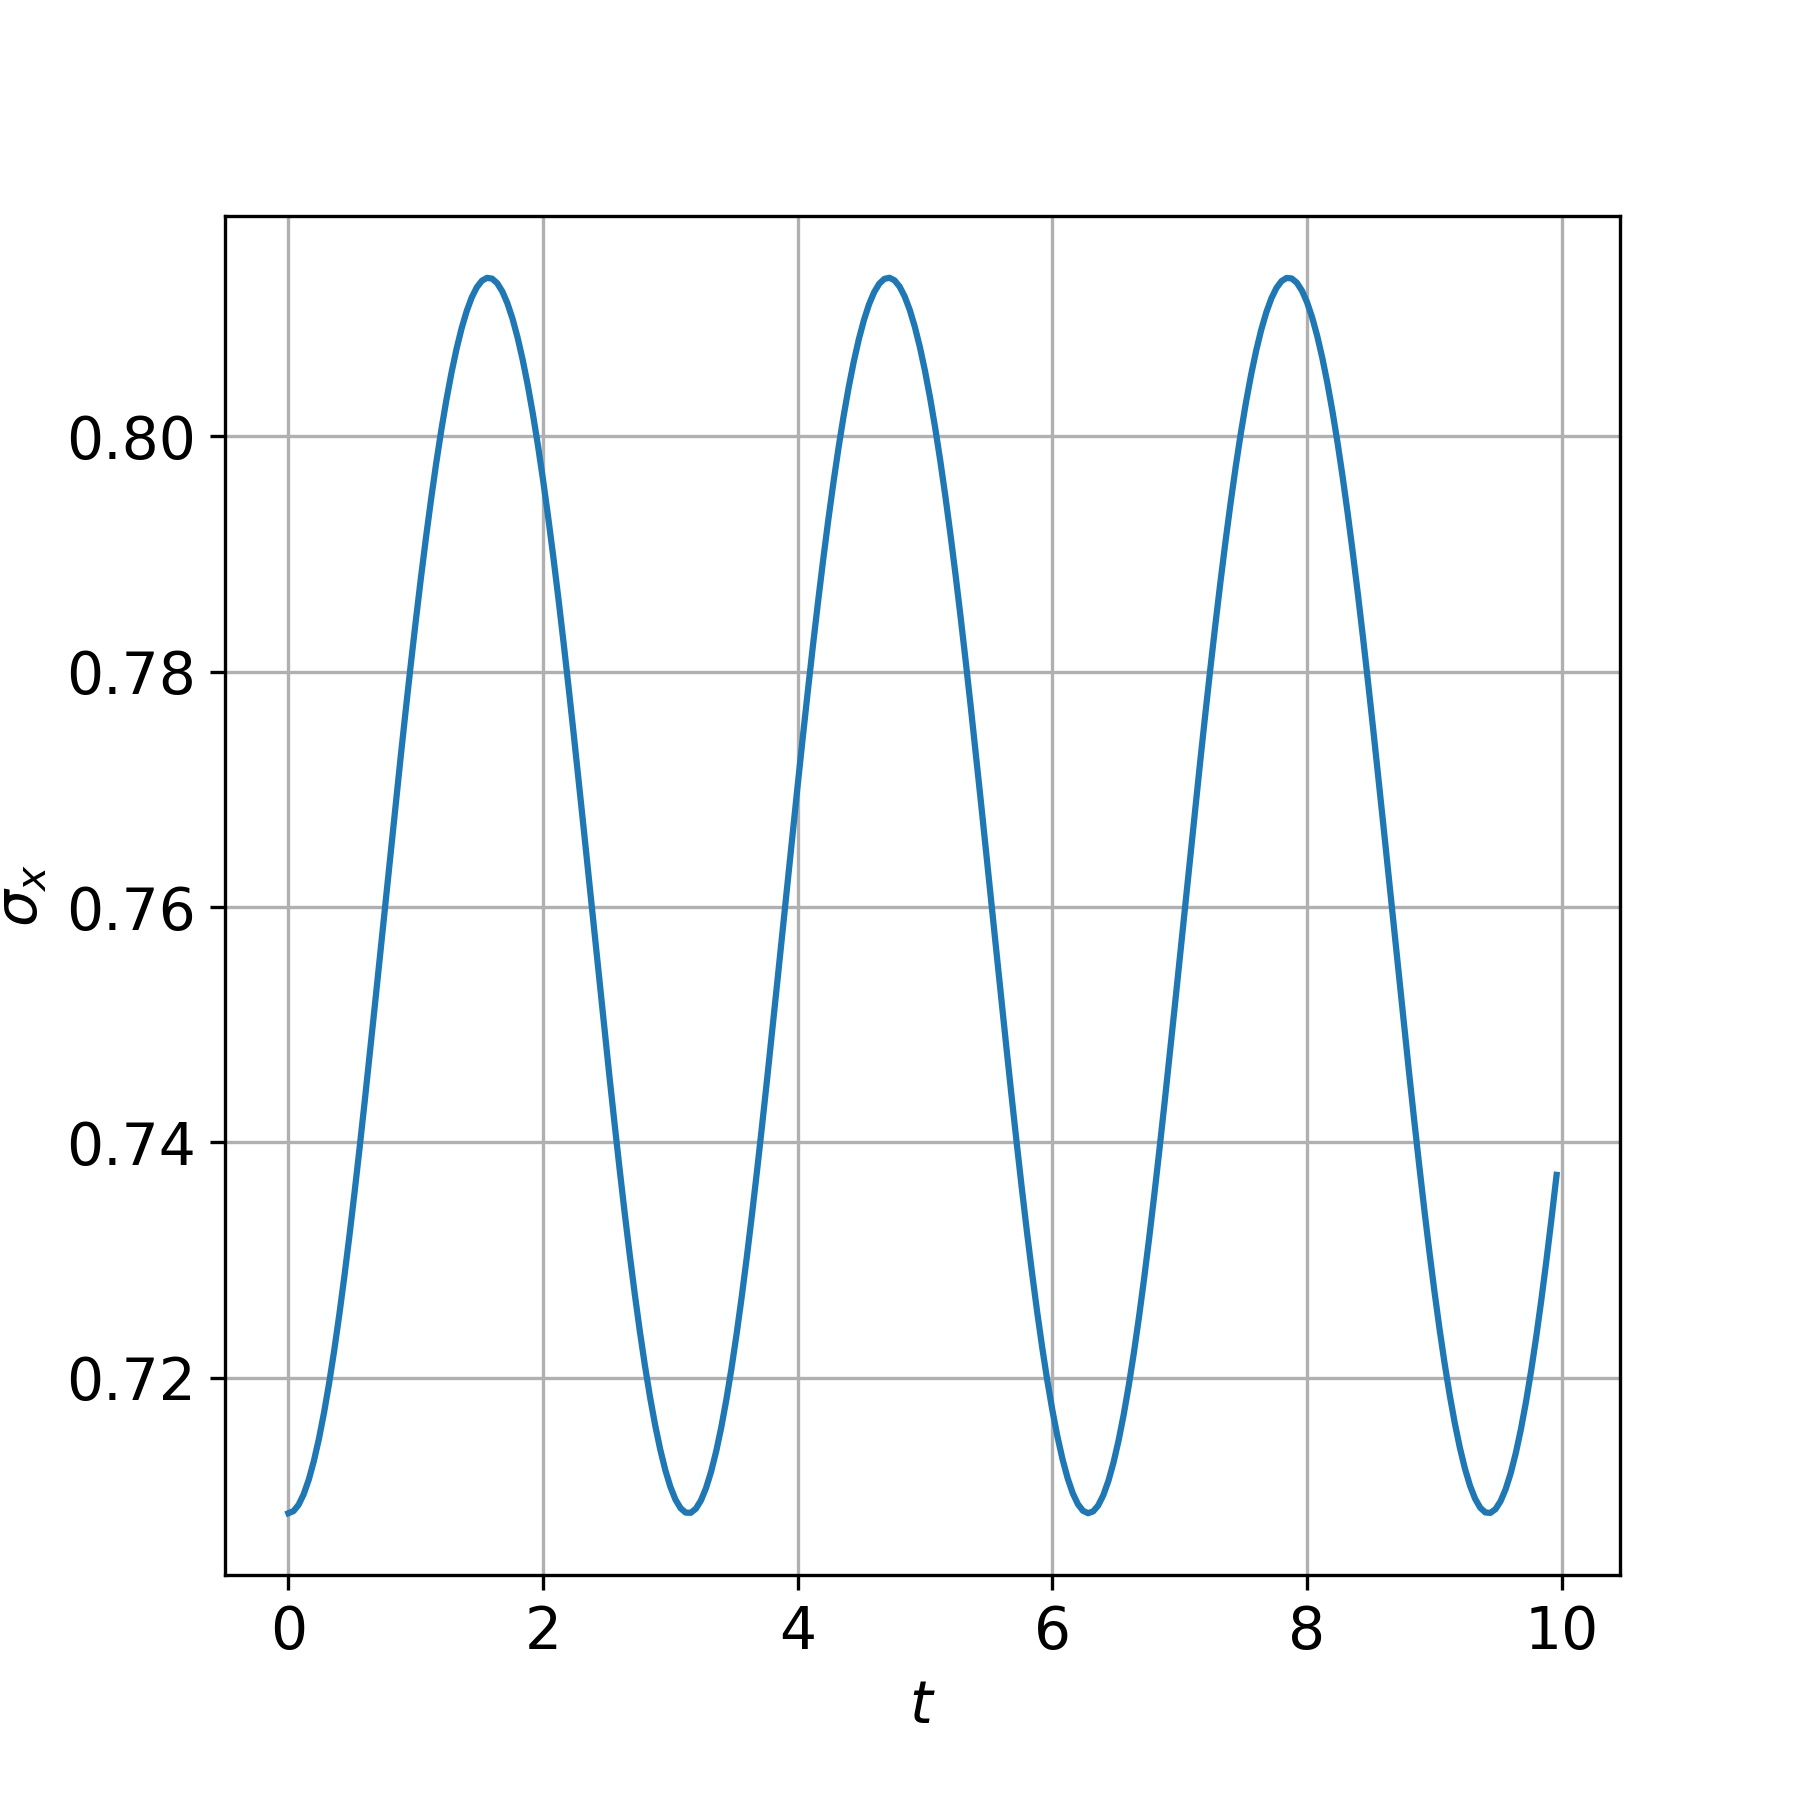
\includegraphics[width=\textwidth]{imgs/sigma_oscillations/sigma_oscillation_isotrop.jpeg}
        \caption{Isotropic case.}
        \label{fig:isotropic-oscillation}
    \end{subfigure}
    \hfill
    \begin{subfigure}[b]{0.45\textwidth}
        \centering
        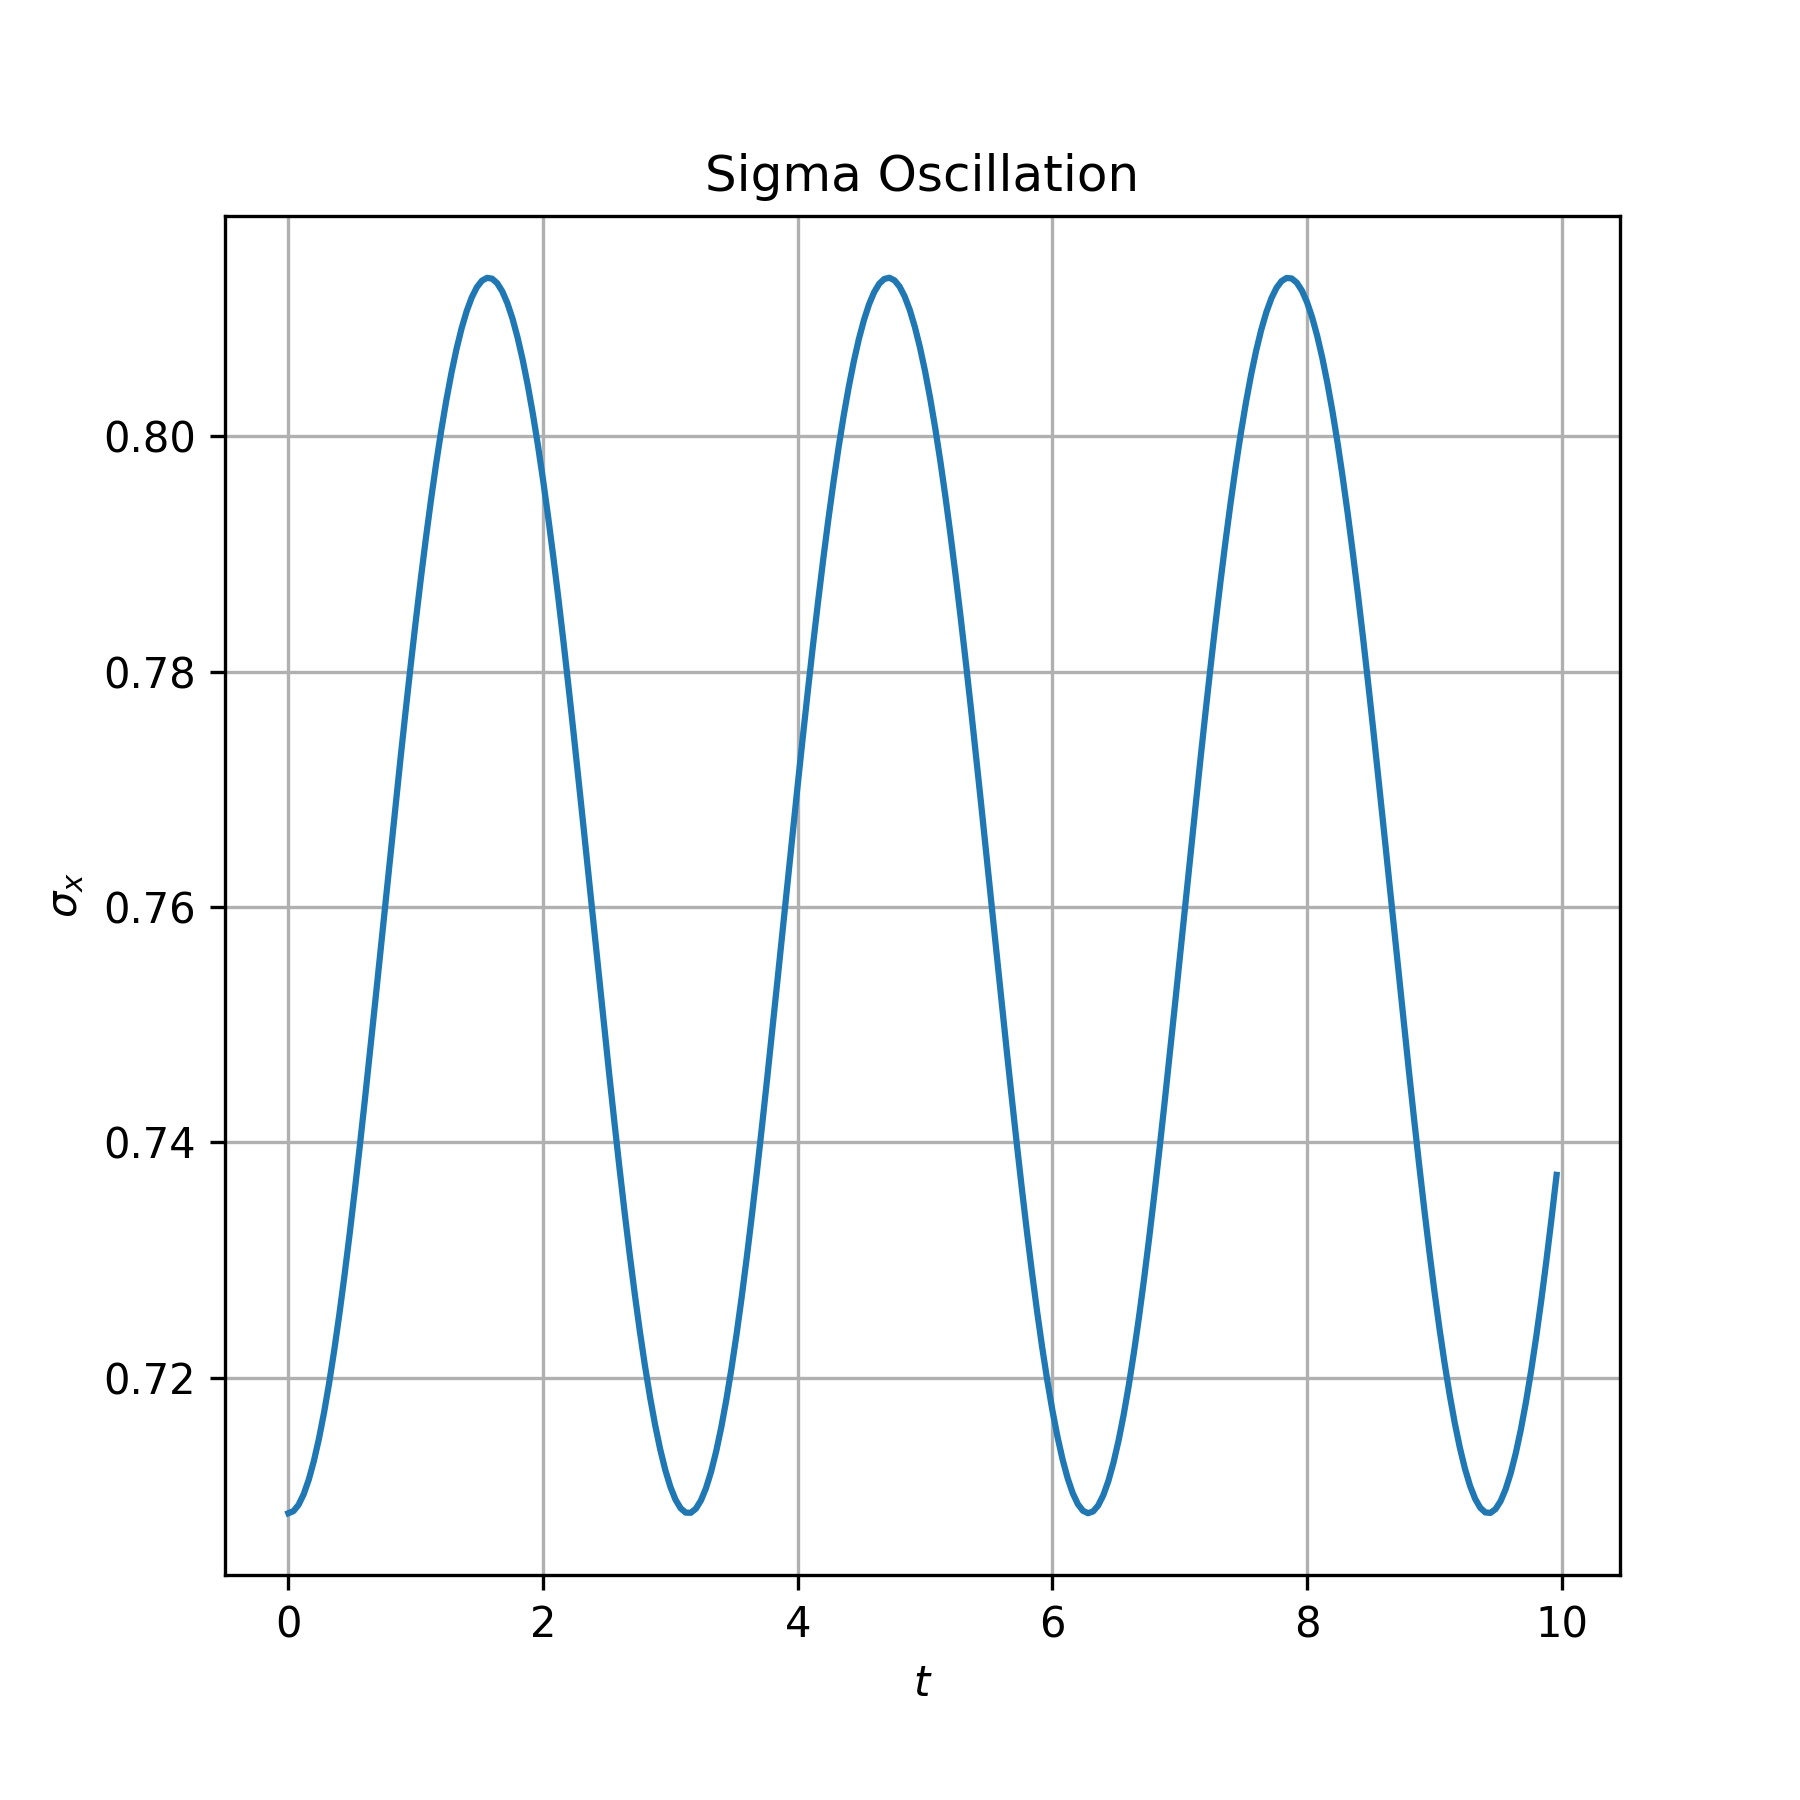
\includegraphics[width=\textwidth]{imgs/sigma_oscillation.jpeg}
        \caption{$y=x$}
        \label{fig:y equals x}
    \end{subfigure}
    
    \caption{Three simple graphs}
    \label{fig:three graphs}
\end{figure}

To test the implementation we simulated the evolution of a Gaussian initial condition inside a symmetric harmonic potential. By defining:
$$
\langle f\rangle=\int_{\mathbb{R}^2} f(\vec{x}) |\psi(\vec{x},t)|^2 \: d\vec{x} \qquad, \qquad \sigma_{x_i}=\sqrt{\langle(x_i-\langle x_i \rangle)^2\rangle}
$$
The evolution of the initial condition is an oscillatory movement of the wave function that expands and contracts inside the harmonic potential. An indicator of the width of the wave function is $\sigma_{x_i}$ along that specific direction. For the previously mentioned case the evolution of the standard deviation from the mean can be found in Figure \ref{fig:isotropic-oscillation}.

The same results can be found in the reference paper \cite{bao1}.

\section{Computation of the ground state}\label{sec:Ground}
\subsection{The problem}
We want now to compute the ground state $\psi_g$ in our harmonic potential which we should take as our initial state before disturbing it with the laser. To do this, we adopt a normalized gradient flow technique used in \cite{bao2}.

\bigskip
The energy of the state where the bosons are described by the wave-function $\psi$ is (see Appendix \eqref{Energy_int}):
$$E=N\int d\mathbf{r}\left(\frac{\hbar^2}{2m}|\nabla\psi(\mathbf{r})|^2+V(\mathbf{r})|\psi(\mathbf{r})|^2+\frac{(N-1)}{2}U_0|\psi(\mathbf{r})|^4\right)$$
where all the quantities have their physical dimension. We turn it into a dimensionless expression following the same procedure as before. We additionally divide by $N$ and use $N-1\approx N$. We thus obtain the dimensionless energy per particle:
$$\mathcal{E}=\int d\mathbf{r}\left(\frac{\varepsilon^2}{2}|\nabla\psi(\mathbf{r})|^2+V(\mathbf{r})|\psi(\mathbf{r})|^2+\frac{\kappa}{2}|\psi(\mathbf{r})|^4\right)$$
Now we consider a solution $\psi(\tau)$ of the equation:
$$\pdv{\psi}{\tau}=-\frac{1}{2}\frac{\delta\mathcal{E}}{\delta\psi}$$
$\psi(\tau)$ will converge to a minimum of $\mathcal{E}$ when $\tau\longrightarrow \infty$. We will assume this to be the ground state $\psi_g$.The factor $\frac{1}{2}$ is irrelevant for this property. But we will see shortly its practical value.\par
Indeed, an immediate computation proves that the previous equation is equivalent to the differential equation:
\begin{equation}\label{eq:gradient}
   \frac{\partial \psi}{\partial \tau}=\frac{\varepsilon}{2} \nabla^{2} \psi-\frac{1}{\varepsilon}\left(V +\kappa|\psi|^{2}\right) \psi 
\end{equation}
and this is nothing but the dimensionless GPE where $t$ has been replaced by an imaginary time $-i\tau$.\par
We need then to integrate \eqref{eq:gradient} and take $\psi_g$ as the value of the solution when $\mathcal{E}$ stops to vary significantly.

\bigskip
An final theoretical remark: it is shown in \cite{bao2} that the chemical potential is given by the expression:
$$\mu=\int d\mathbf{r}\left(\frac{\varepsilon^2}{2}|\nabla\psi(\mathbf{r})|^2+V(\mathbf{r})|\psi(\mathbf{r})|^2+\kappa|\psi(\mathbf{r})|^4\right)=\mathcal{E}+\int d\mathbf{r}\frac{\kappa}{2}|\psi(\mathbf{r})|^4$$


\subsection{Integration scheme}
We will use the same numerical integration approach. The two equations of the time-splitting are now:
\begin{equation}\label{eq:Agradient}
   \frac{\partial f}{\partial \tau}(\mathbf{r},\tau)=-\frac{1}{\varepsilon}\left(V +\kappa|f(\mathbf{r},\tau)|^{2}\right) f(\mathbf{r},\tau)
\end{equation}
\begin{equation}\label{eq:Bgradient}
   \frac{\partial f}{\partial \tau}(\mathbf{r},\tau)=\frac{\varepsilon}{2} \nabla^{2} f(\mathbf{r},\tau)
\end{equation}
Equation \eqref{eq:Bgradient} can be integrated in the same way as \eqref{eqB} using the DFT. However, equation \eqref{eq:Agradient} no longer preserves the modulus of $f(\mathbf{r},\tau)$ as did \eqref{eqA} and cannot be integrated in the same way. An exact solution can still be obtained (see \cite{bao2} p. 1683). Writing $\varphi_\tau$ the flow of the equation, the solution is given by:
$$
\varphi_\tau(u)(\mathbf{r}) = \left\{
    \begin{aligned}
        & \sqrt{\frac{V(\mathbf{r})}{(V(\mathbf{r})+\kappa u^2)e^{2V(\mathbf{r})\tau/\varepsilon}-\kappa u^2}}~u & \text{   if } V(\mathbf{r})\neq 0 \\
        & \frac{1}{\sqrt{1+2\kappa u^2 \tau/\varepsilon}}~u & \text{   if } V(\mathbf{r})= 0
    \end{aligned}
\right.
$$
It should be observed that these two equations do not preserve norm. So, following \cite{bao2}, we add a normalization step in our scheme. This corresponds to solving the minimization problem with the constraint:
$$\int d\mathbf{r}\psi=\text{cste}$$
which we take to be 1. Our integration scheme becomes then:
$$
\begin{aligned}
\psi^{n,(1)}_{ij} & =\left\{
    \begin{aligned}
        & \sqrt{\frac{V(x_i,y_j)}{(V(x_i,y_j)+\kappa |\psi^n_{ij}|^2)e^{V(\mathbf{r})d\tau/\varepsilon}-\kappa |\psi^n_{ij}|^2}}~\psi^n_{ij} & \text{   if } V(x_i,y_j)\neq 0 \\
        & \frac{1}{\sqrt{1+\kappa |\psi^n_{ij}|^2 d\tau/\varepsilon}}~\psi^n_{ij} & \text{   if } V(x_i,y_j)= 0
    \end{aligned}
\right. \\
\psi^{n,(2)} & =\mathcal{F}_D^{-1}\left[\left\{\exp{-\frac{\varepsilon}{2}\left(\mu_{x,k}^2+\mu_{y,l}^2\right)d\tau}\mathcal{F}_D\left[\psi^{n,(1)}\right]_{kl}\right\}_{kl}\right] \\
\psi^{n,(3)}_{ij} & =\left\{
    \begin{aligned}
        & \sqrt{\frac{V(x_i,y_j)}{(V(x_i,y_j)+\kappa |\psi^{n,(2)}_{ij}|^2)e^{V(\mathbf{r})d\tau/\varepsilon}-\kappa |\psi^{n,(2)}_{ij}|^2}}~\psi^{n,(2)}_{ij} & \text{   if } V(x_i,y_j)\neq 0 \\
        & \frac{1}{\sqrt{1+\kappa |\psi^{n,(2)}_{ij}|^2 d\tau/\varepsilon}}~\psi^{n,(2)}_{ij} & \text{   if } V(x_i,y_j)= 0
    \end{aligned}
\right.\\
\psi^{n+1} & =\frac{1}{||\psi^{n,(3)}||_2}\psi^{n,(3)}
\end{aligned}
$$


\subsection{Numerical results}

\begin{figure}
    \centering
    \begin{subfigure}[b]{0.45\textwidth}
        \centering
        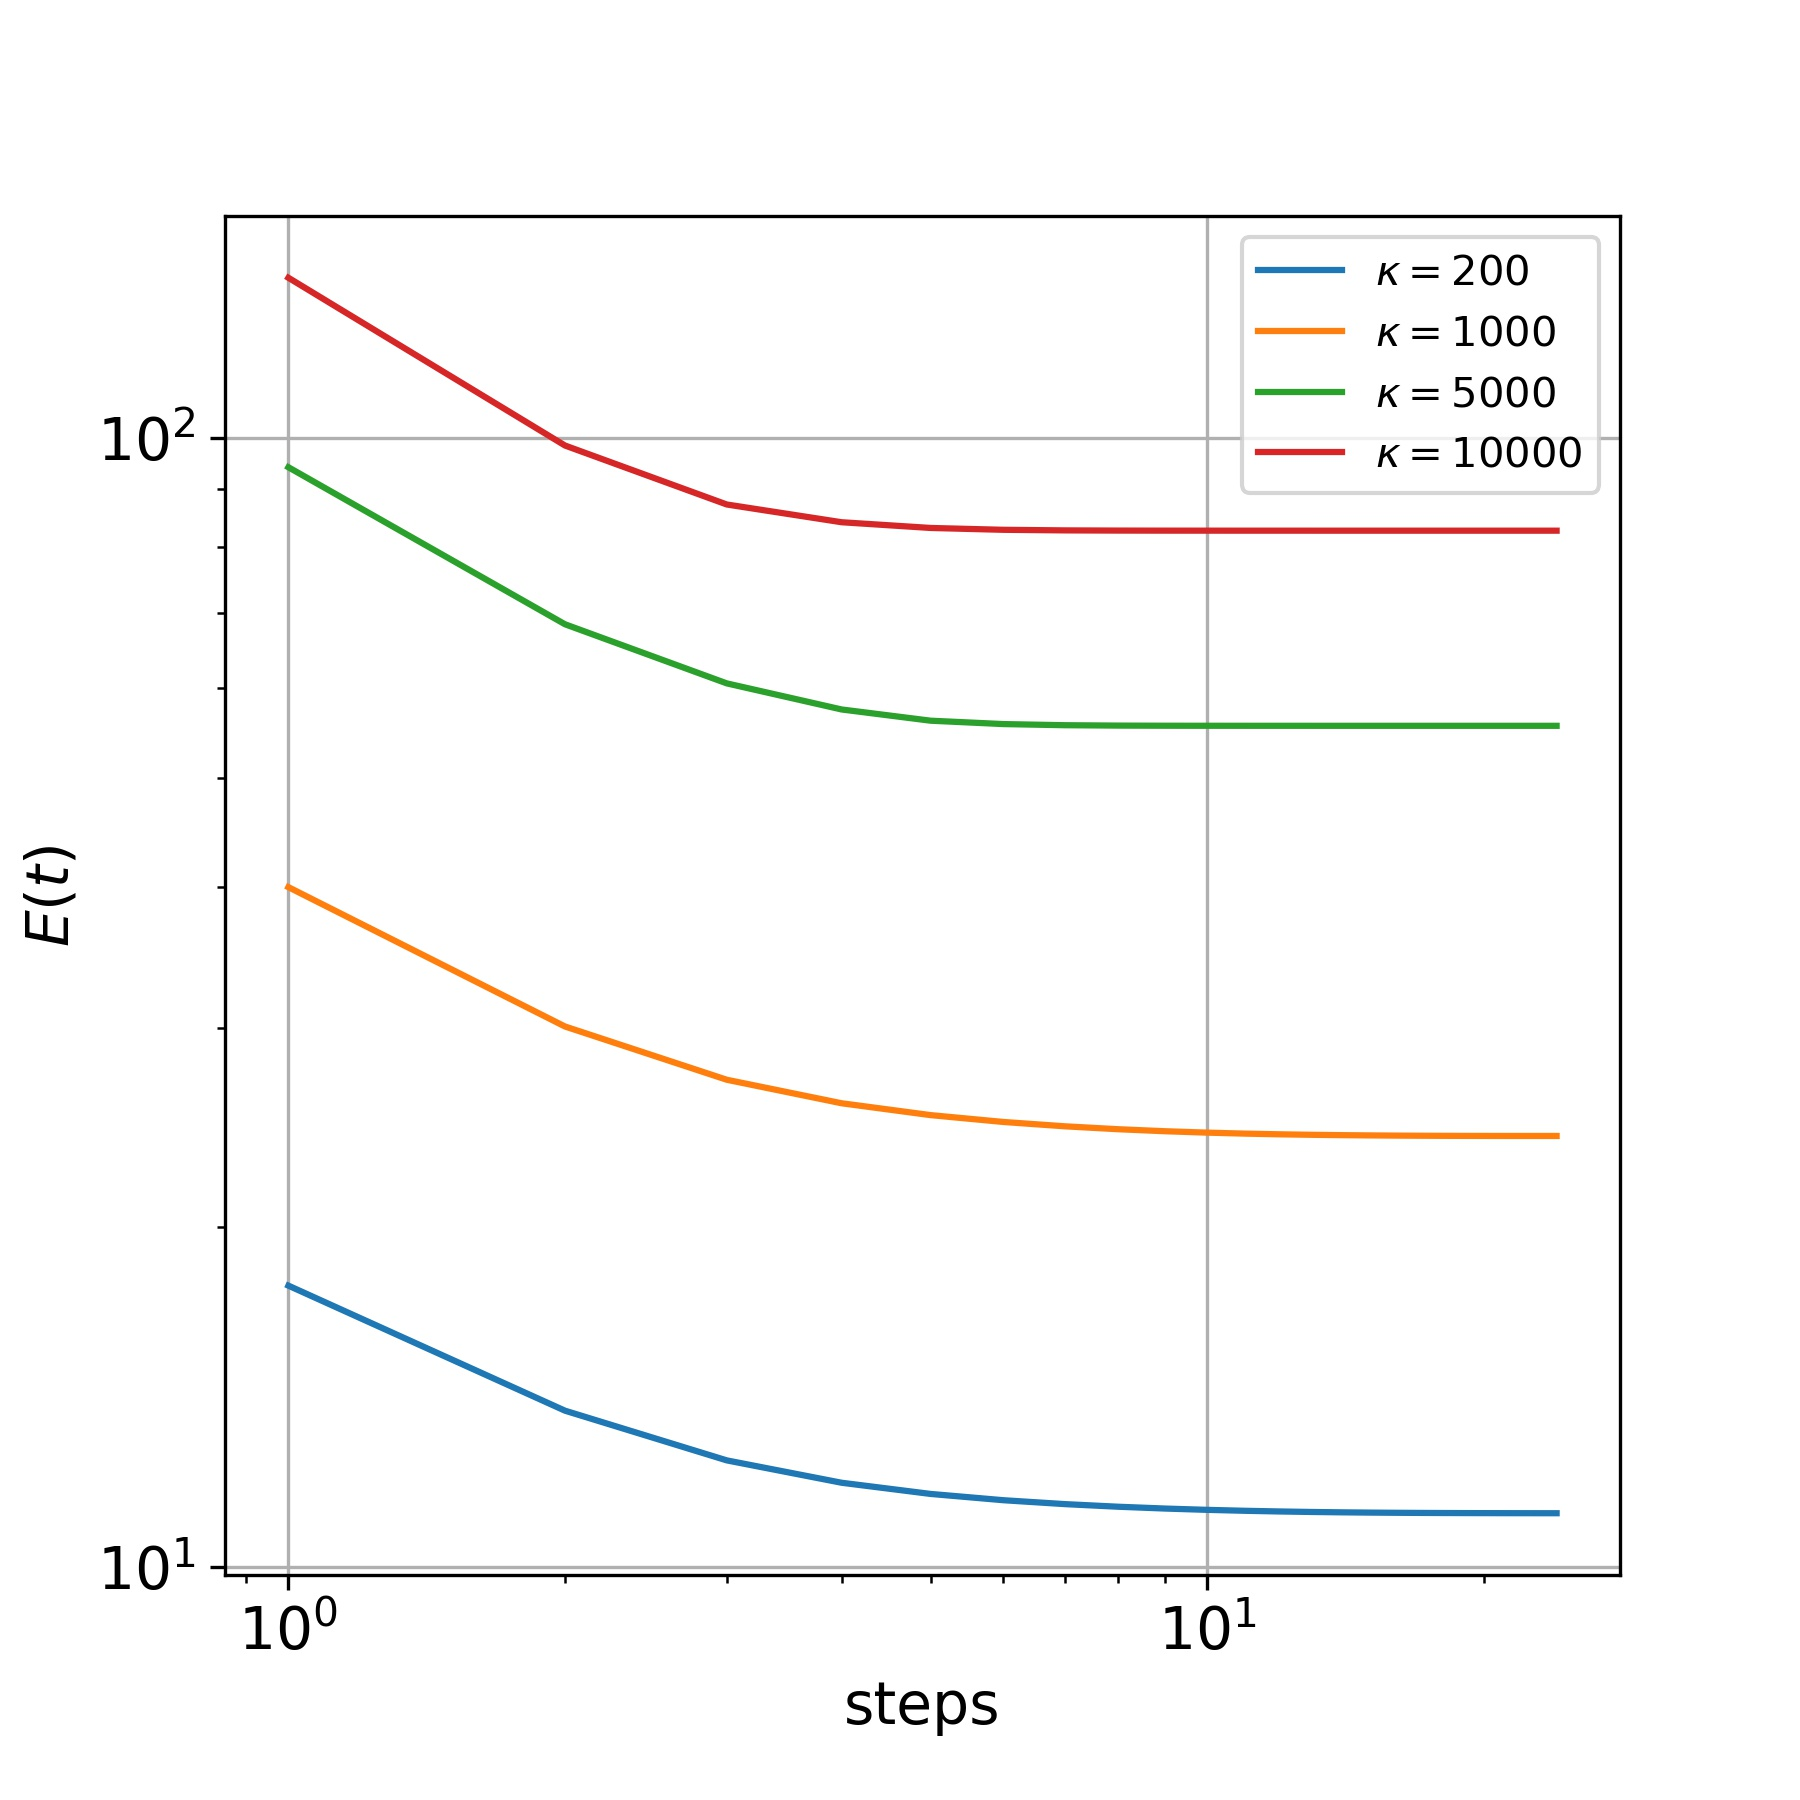
\includegraphics[width=\textwidth]{imgs/gradient_descent/E_convergence.jpeg}
        \caption{Energy convergence for different $\kappa$.}
        \label{fig:energy-convergence}
    \end{subfigure}
    \hfill
    \begin{subfigure}[b]{0.45\textwidth}
        \centering
        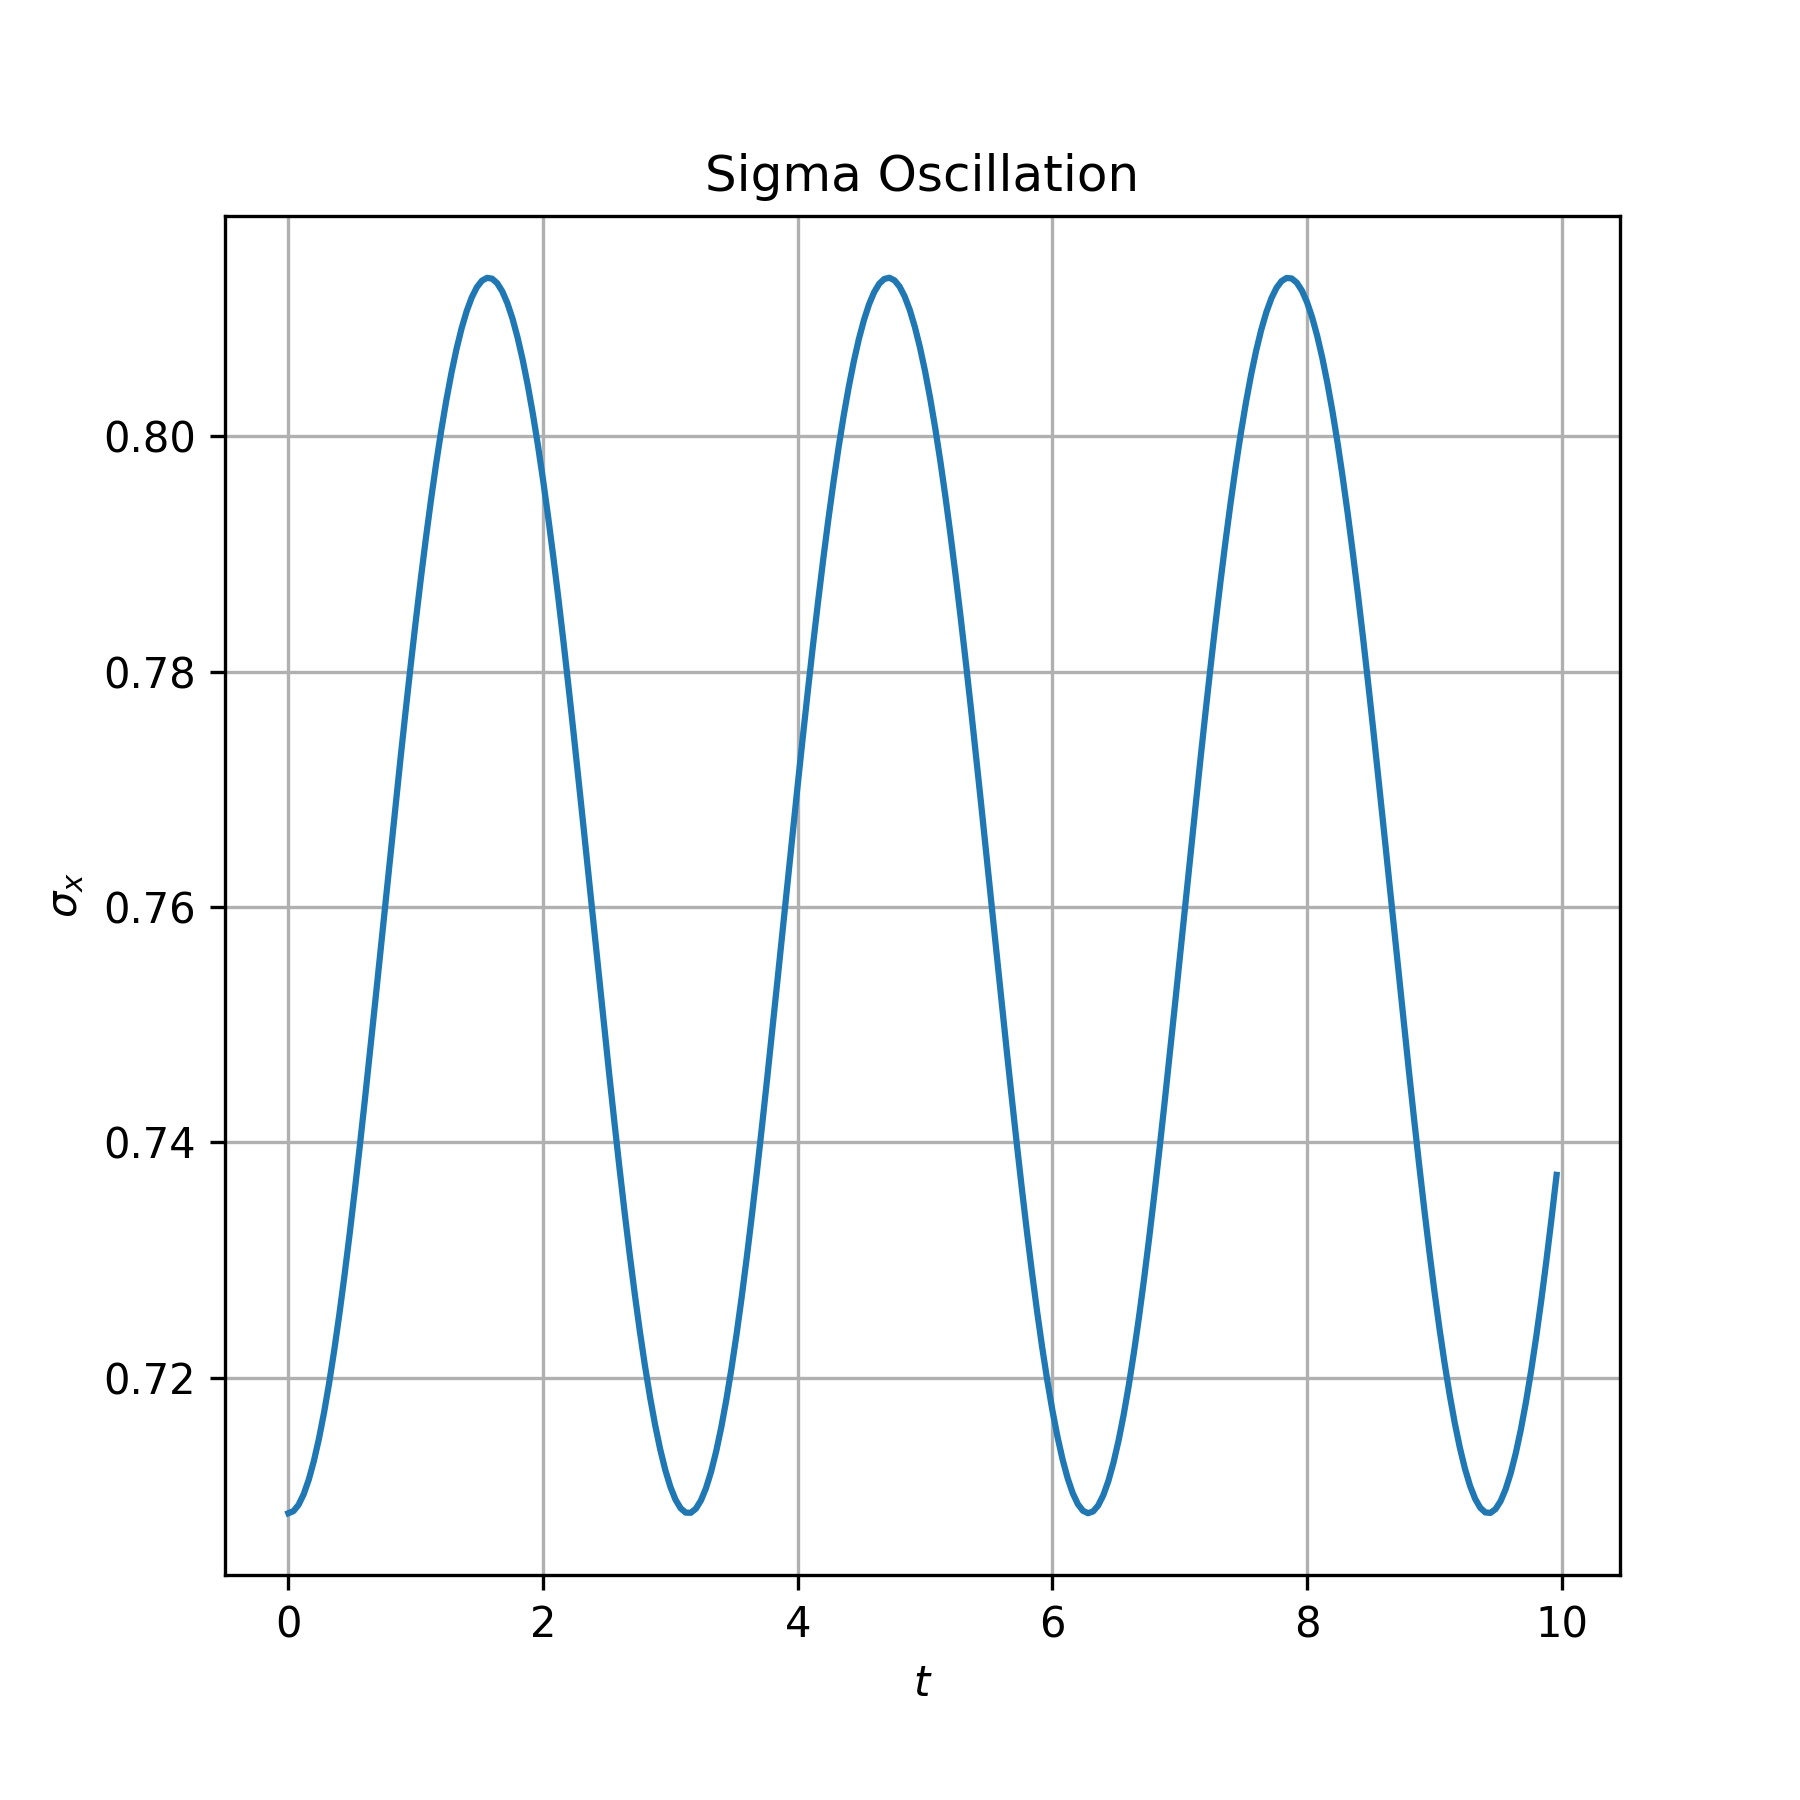
\includegraphics[width=\textwidth]{imgs/sigma_oscillation.jpeg}
        \caption{$y=x$}
        \label{fig:y equals x}
    \end{subfigure}
    
    \caption{Three simple graphs}
    \label{fig:gradient-descent-results}
\end{figure}



\section{Vortex pairs}\label{sec:Vortex}
\subsection{The problem}
We now want to simulate the experiment in which we move a laser in the gas chamber. Our initial state is the ground state computed with the method presented in the previous section:
$$\psi(t=0)=\psi_g$$
And the potential has the form:
$$
V=\frac{1}{2}(x^2+\gamma_y y^2)+w_0 e^{-\delta\left((x-v t)^2+y^2\right)}
$$
with $w_0,\delta,v \neq 0$.

\subsection{Integration scheme}
The important difference from section \ref{sec:Static} is that now $V$ is not static and cannot be integrated analytically on finite time intervals. We will use the approximation:
$$V(t)\approx V(t_n) \qquad,\qquad \text{for  } t\in\left[t_n,t_{n+1}\right]$$
This however will increase the error of the time discretization. Indeed, let us write $\tilde{\varphi}_t^A$ the flow with the approximation of constant $V$. We have:
$$
\begin{aligned}
    \varphi^A_{dt}(u) &=\exp{-\frac{i}{\varepsilon}\left(\int_0^{dt} V(\mathbf{r},s)ds +\kappa|u|^{2}dt\right)}u\\
    &=\exp{-\frac{i}{\varepsilon}\left(\int_0^{dt} V(\mathbf{r},0)+\mathcal{O}(s)ds +\kappa|u|^{2}dt\right)}u\\
    &=e^{-\frac{i}{\varepsilon}\left(V(\mathbf{r},0) +\kappa|u|^{2}\right)dt}e^{\mathcal{O}(dt^2)}u\\
    &=e^{-\frac{i}{\varepsilon}\left(V(\mathbf{r},0) +\kappa|u|^{2}\right)dt}\left(1+\mathcal{O}(dt^2)\right)u\\
    &=e^{-\frac{i}{\varepsilon}\left(V(\mathbf{r},0) +\kappa|u|^{2}\right)dt}u+\left(1+\mathcal{O}(dt)\right)\mathcal{O}(dt^2)u\\
    &=\tilde{\varphi}_ {dt}^A+\mathcal{O}(dt^2)
\end{aligned}
$$
And so:
$$\varphi^{A+B}_{dt}(u)=\tilde{\varphi}^A_{dt/2}\circ\tilde{\varphi}^B_{dt}\circ\tilde{\varphi}^A_{dt/2}(u)+r_\text{DFT}(M_x,M_y)+\mathcal{O}(dt^2)$$
instead of $\mathcal{O}(dt^3)$.

\bigskip
Keeping in mind this loss of precision, our integration scheme is sensibly the same as in section \ref{sec:Static}:
$$
\begin{aligned}
\psi^{n,(1)}_{ij}&=\exp{-\frac{i}{\varepsilon}\left(V(x_i,y_j,t_n)+\kappa|\psi^n_{ij}|^{2}\right)\frac{dt}{2}}\psi^n_{ij}\\
\psi^{n,(2)}&=\mathcal{F}_D^{-1}\left[\left\{\exp{-i\frac{\varepsilon}{2}\left(\mu_{x,k}^2+\mu_{y,l}^2\right)dt}\mathcal{F}_D\left[\psi^{n,(1)}\right]_{kl}\right\}_{kl}\right]\\
\psi^{n+1}_{ij}&=\exp{-\frac{i}{\varepsilon}\left(V(x_i,y_j,t_n)+\kappa|\psi^{n,(2)}_{ij}|^{2}\right)\frac{dt}{2}}\psi^{n,(2)}_{ij}
\end{aligned}
$$


\subsection{Numerical results}

\begin{figure}
\centering

\begin{subfigure}[b]{.45\linewidth}
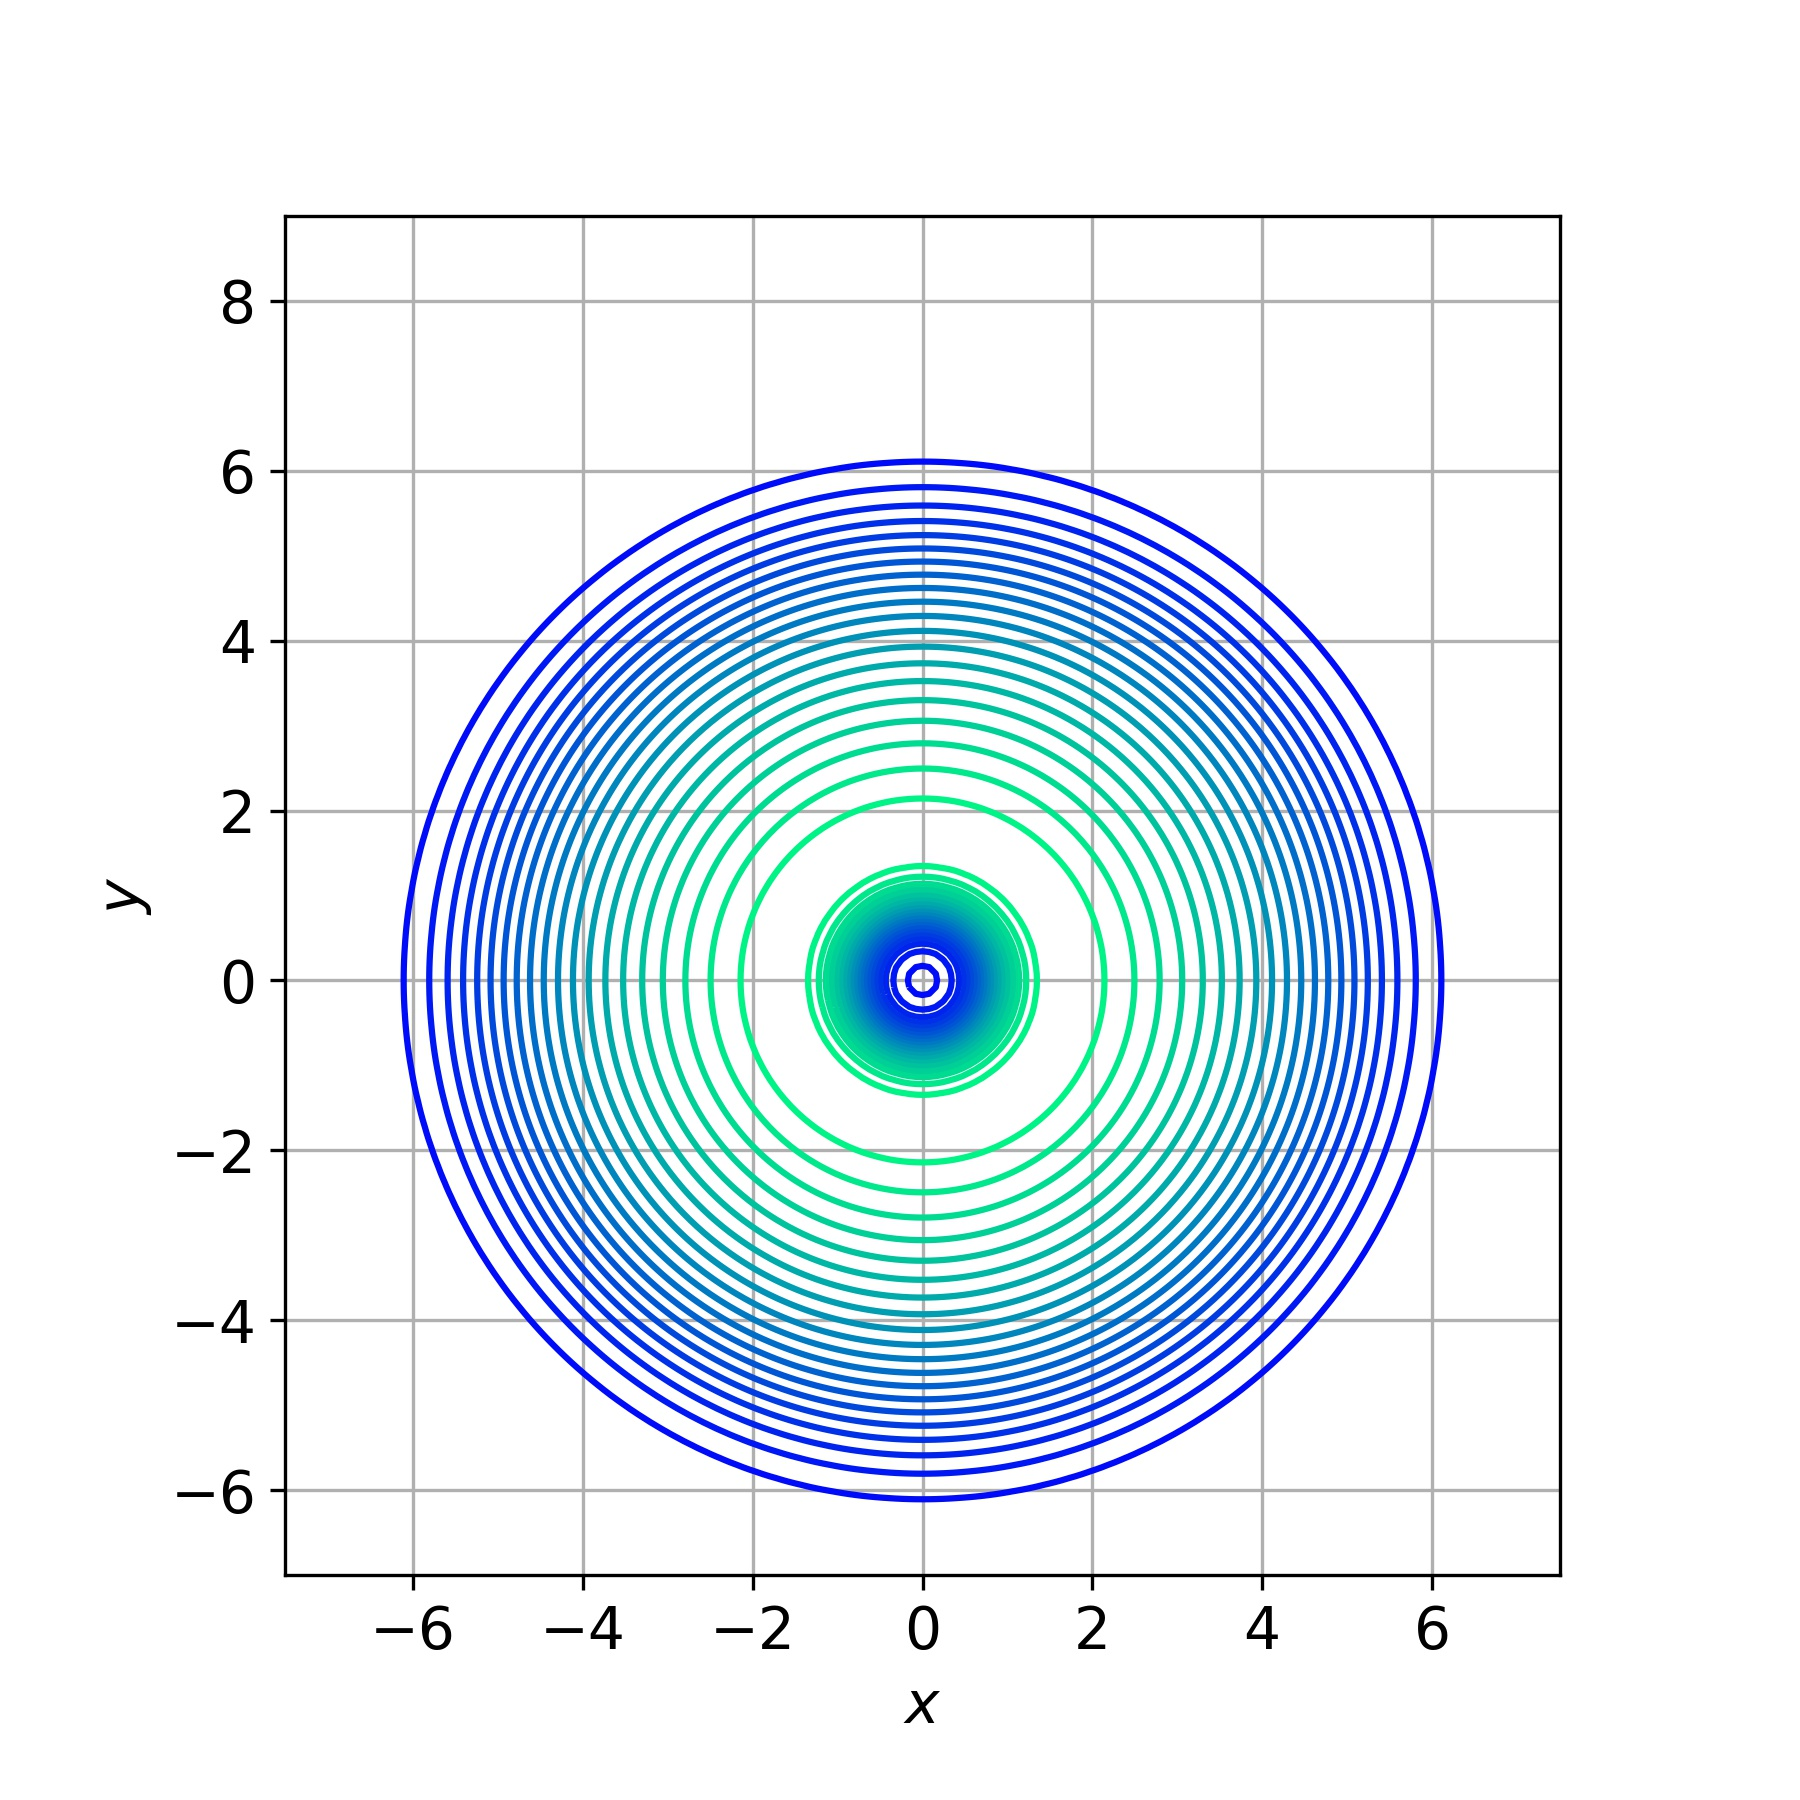
\includegraphics[width=\linewidth]{imgs/vortex_contour/contour_vortices_0.jpeg}
\caption{$t = 0.0$}\label{fig:gull}
\end{subfigure}
\begin{subfigure}[b]{.45\linewidth}
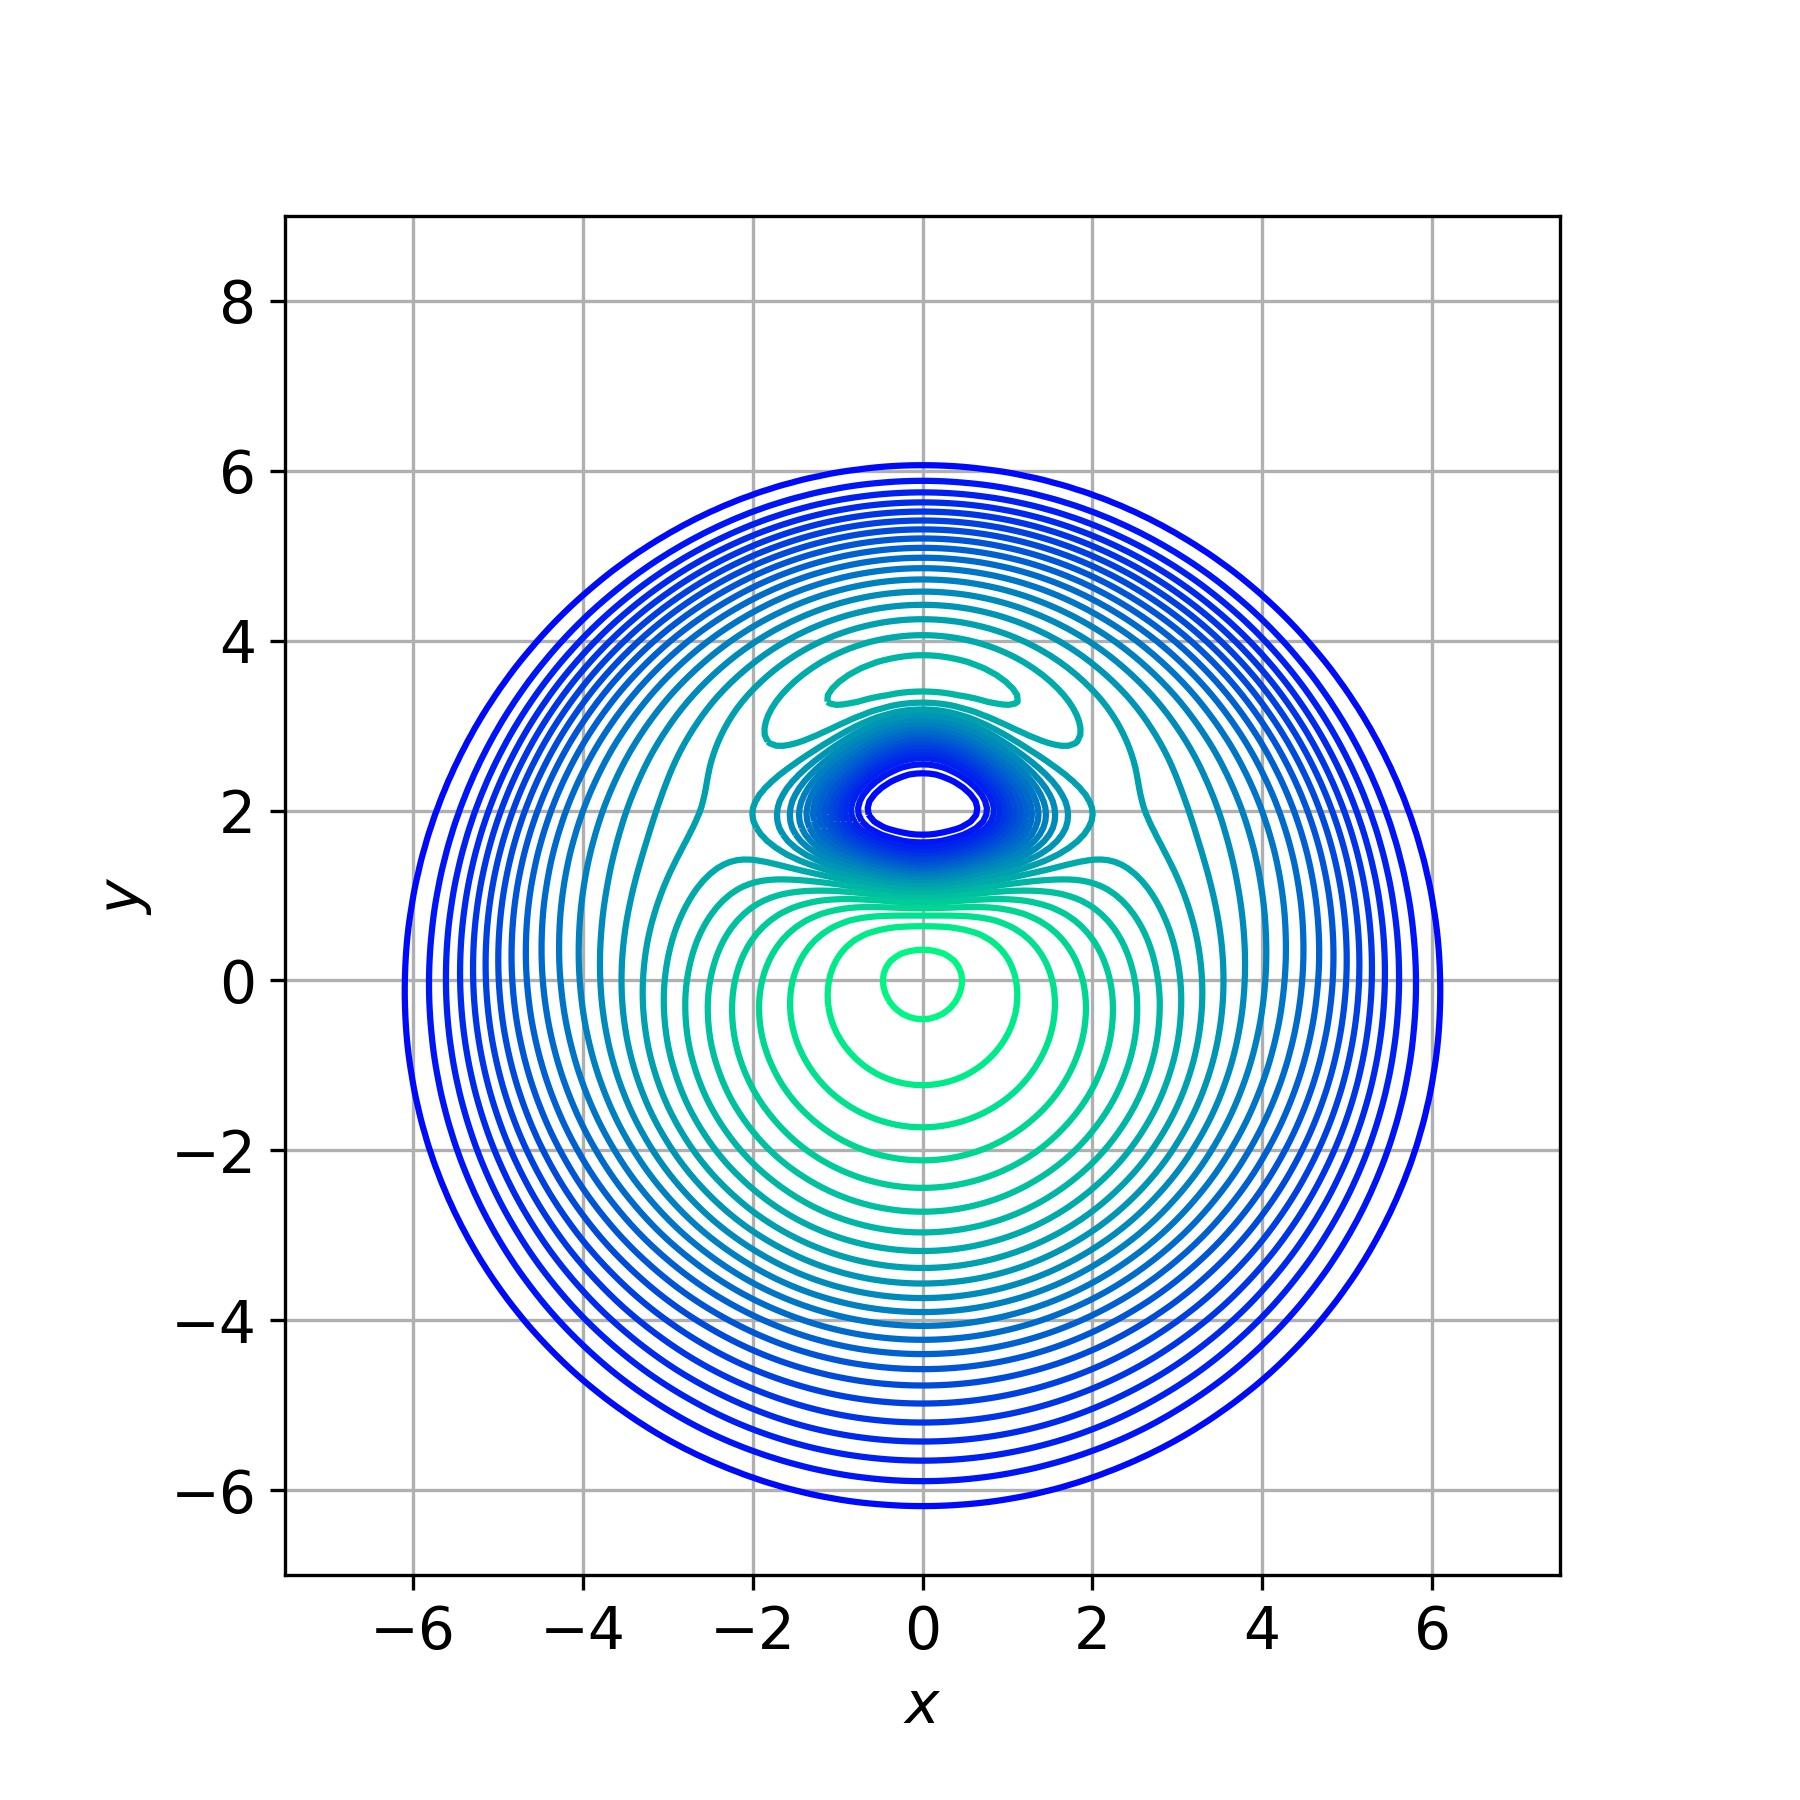
\includegraphics[width=\linewidth]{imgs/vortex_contour/contour_vortices_20.jpeg}
\caption{$t = 0.2$}\label{fig:tiger}
\end{subfigure}

\begin{subfigure}[b]{.45\linewidth}
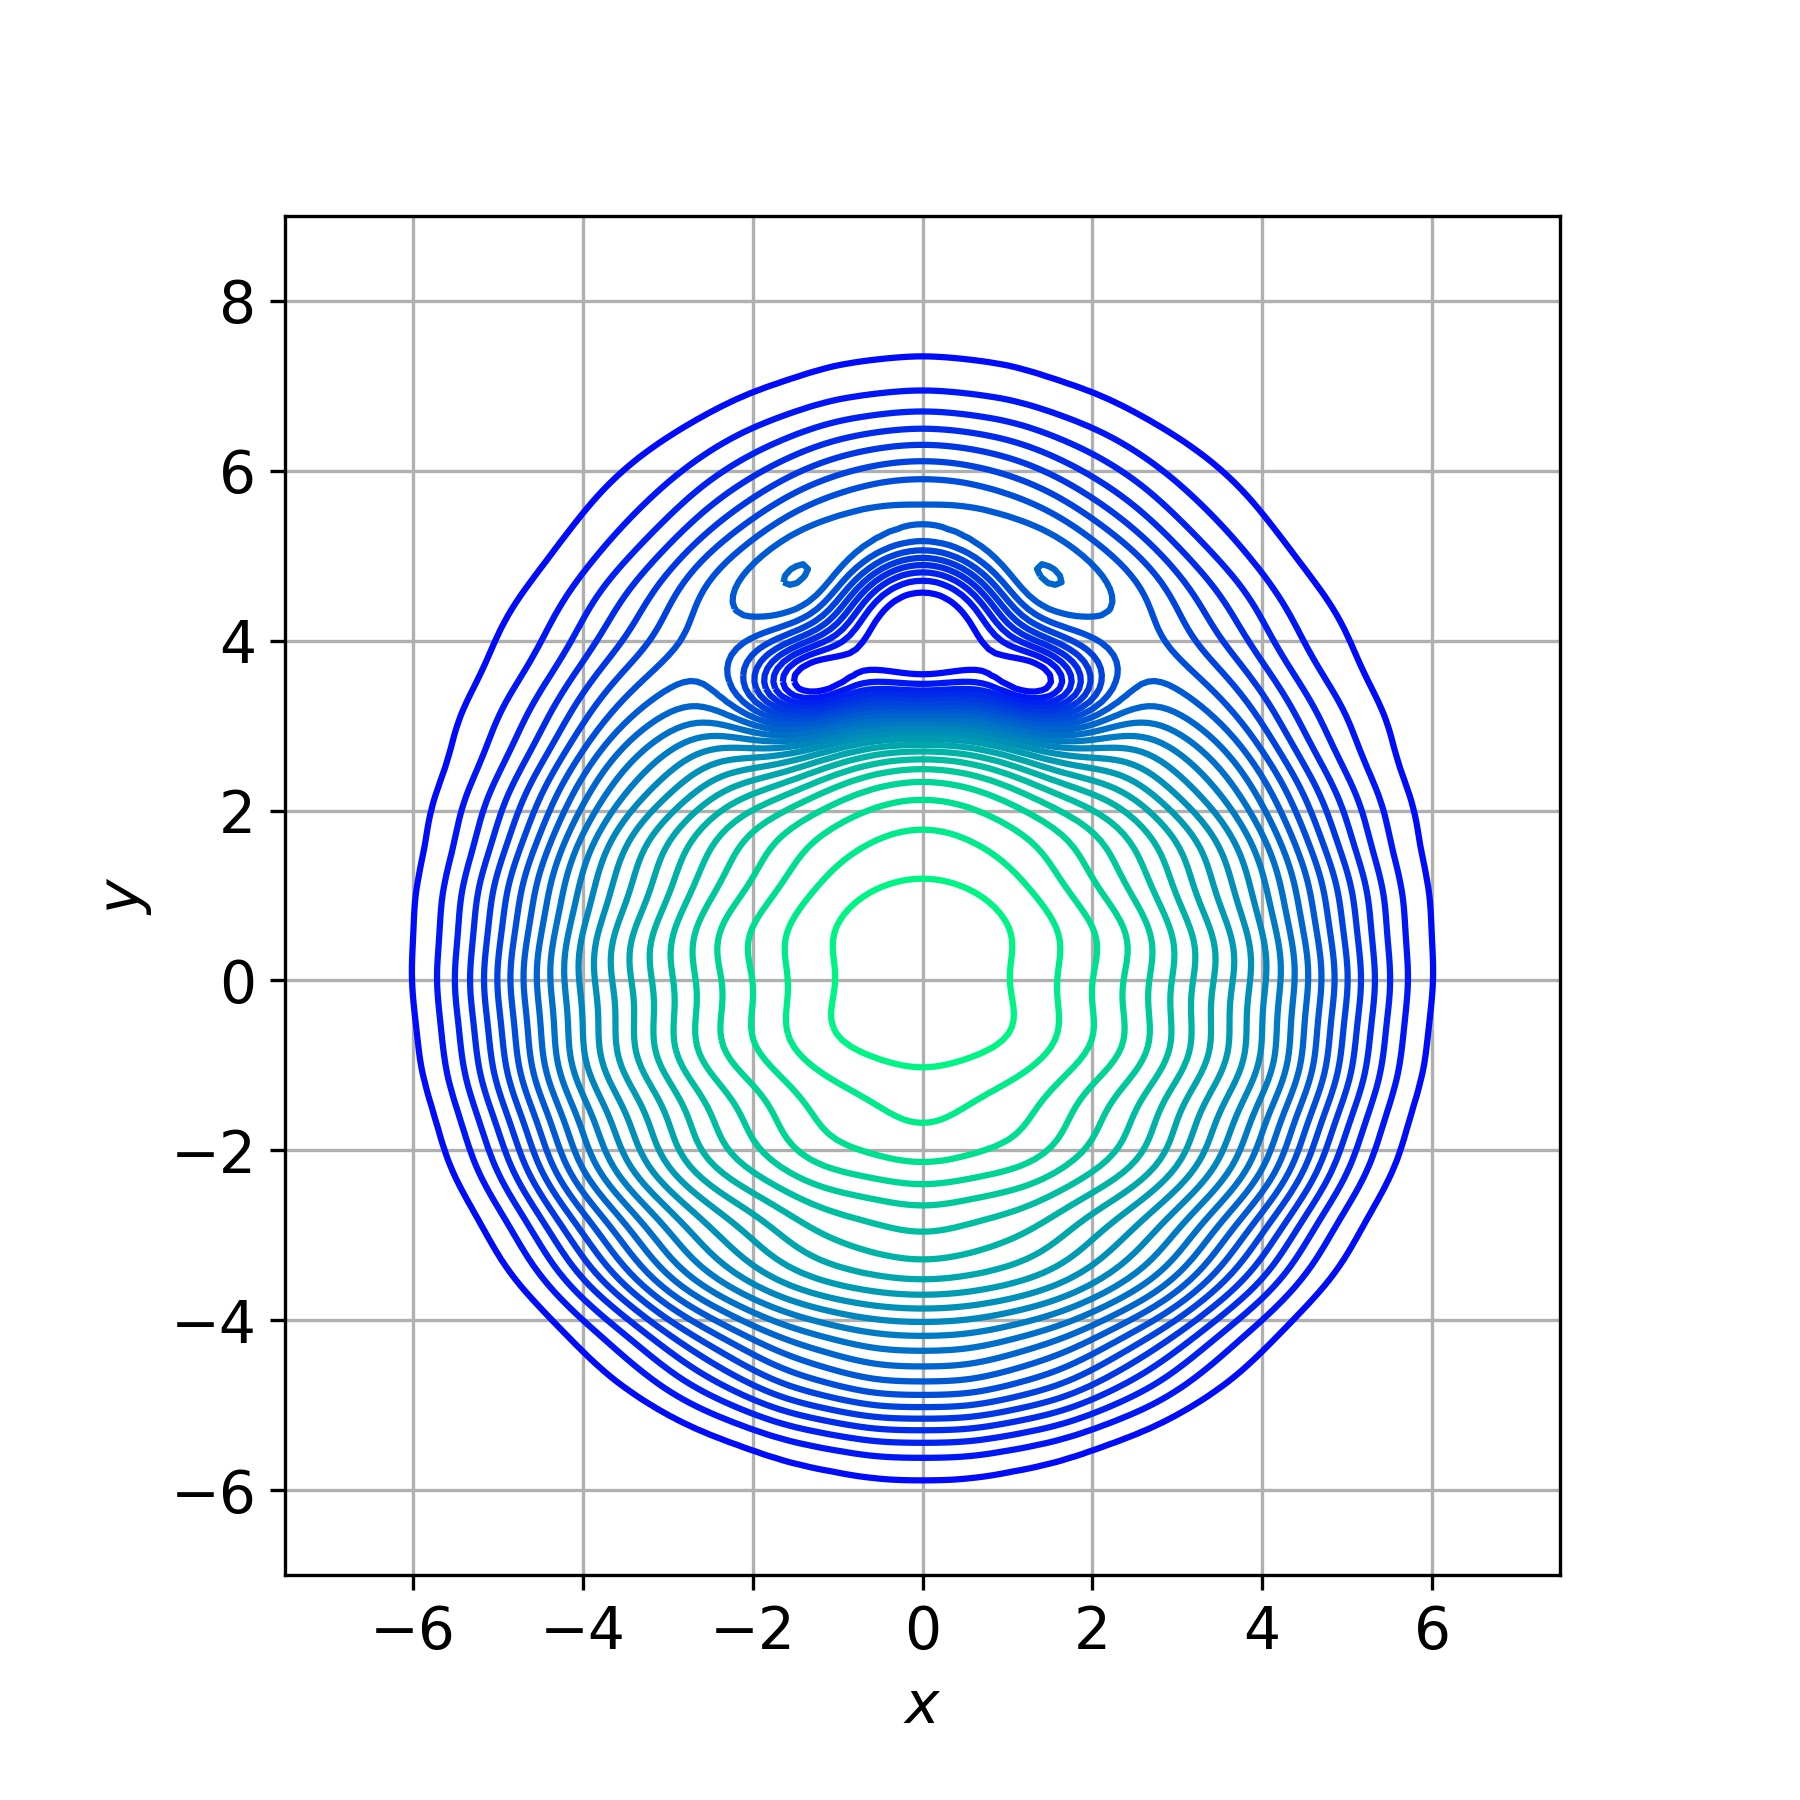
\includegraphics[width=\linewidth]{imgs/vortex_contour/contour_vortices_40.jpeg}
\caption{$t = 0.4$}\label{fig:gull}
\end{subfigure}
\begin{subfigure}[b]{.45\linewidth}
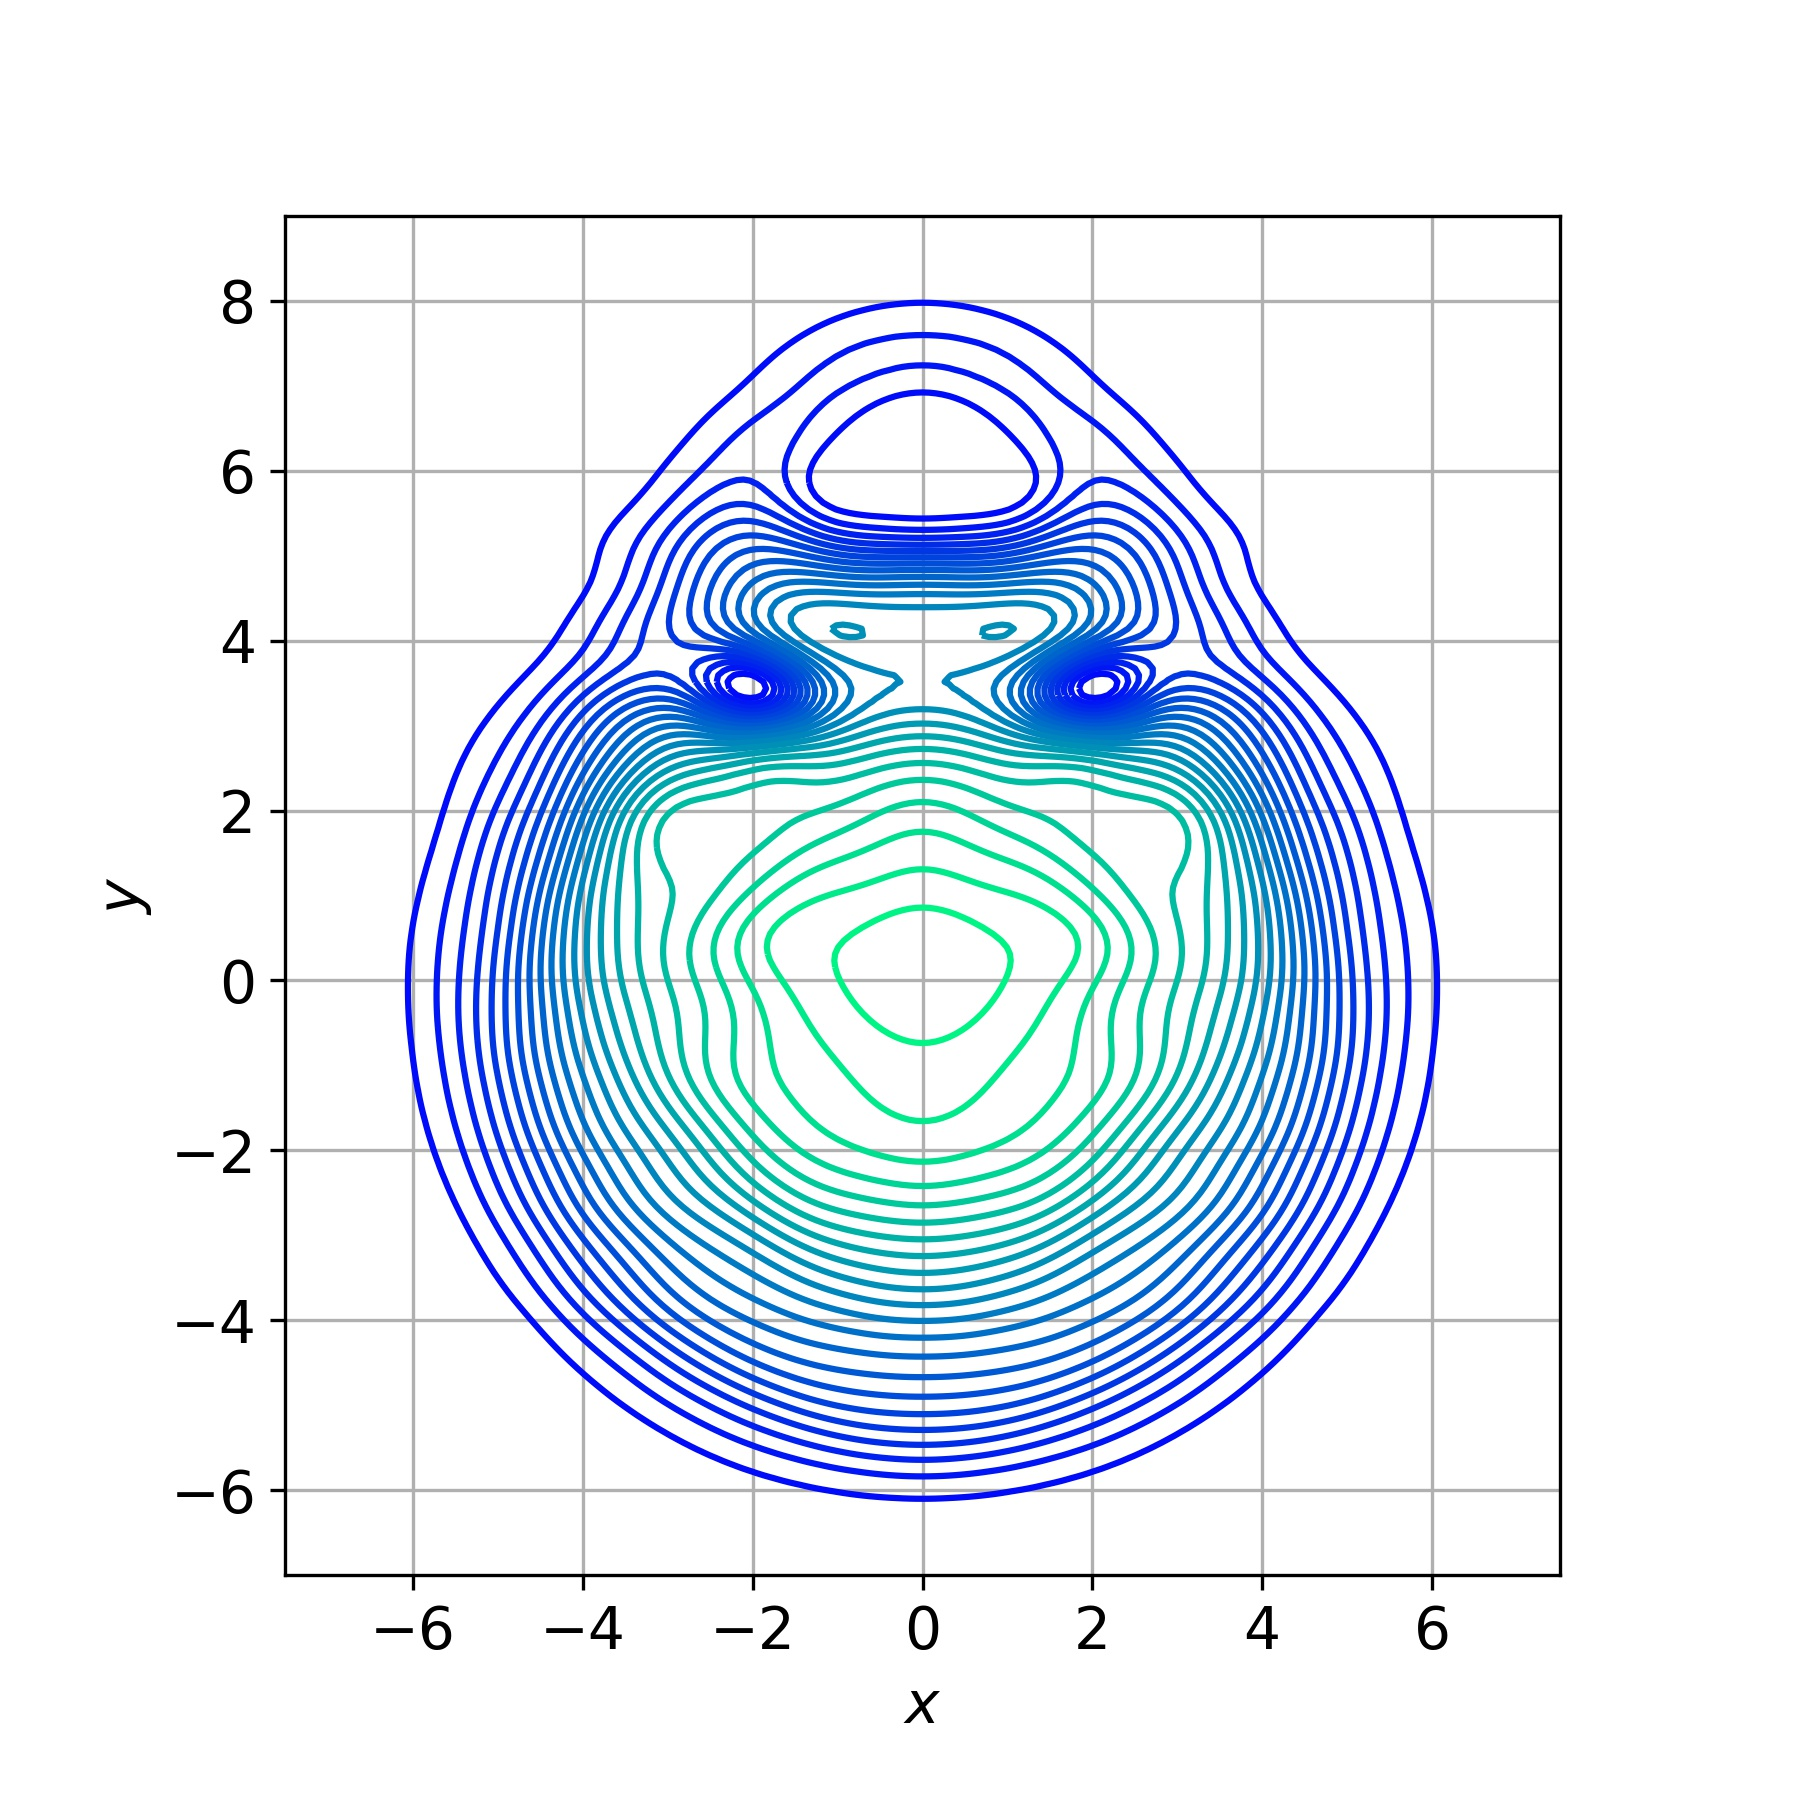
\includegraphics[width=\linewidth]{imgs/vortex_contour/contour_vortices_60.jpeg}
\caption{$t = 0.6$}\label{fig:tiger}
\end{subfigure}

\begin{subfigure}[b]{.45\linewidth}
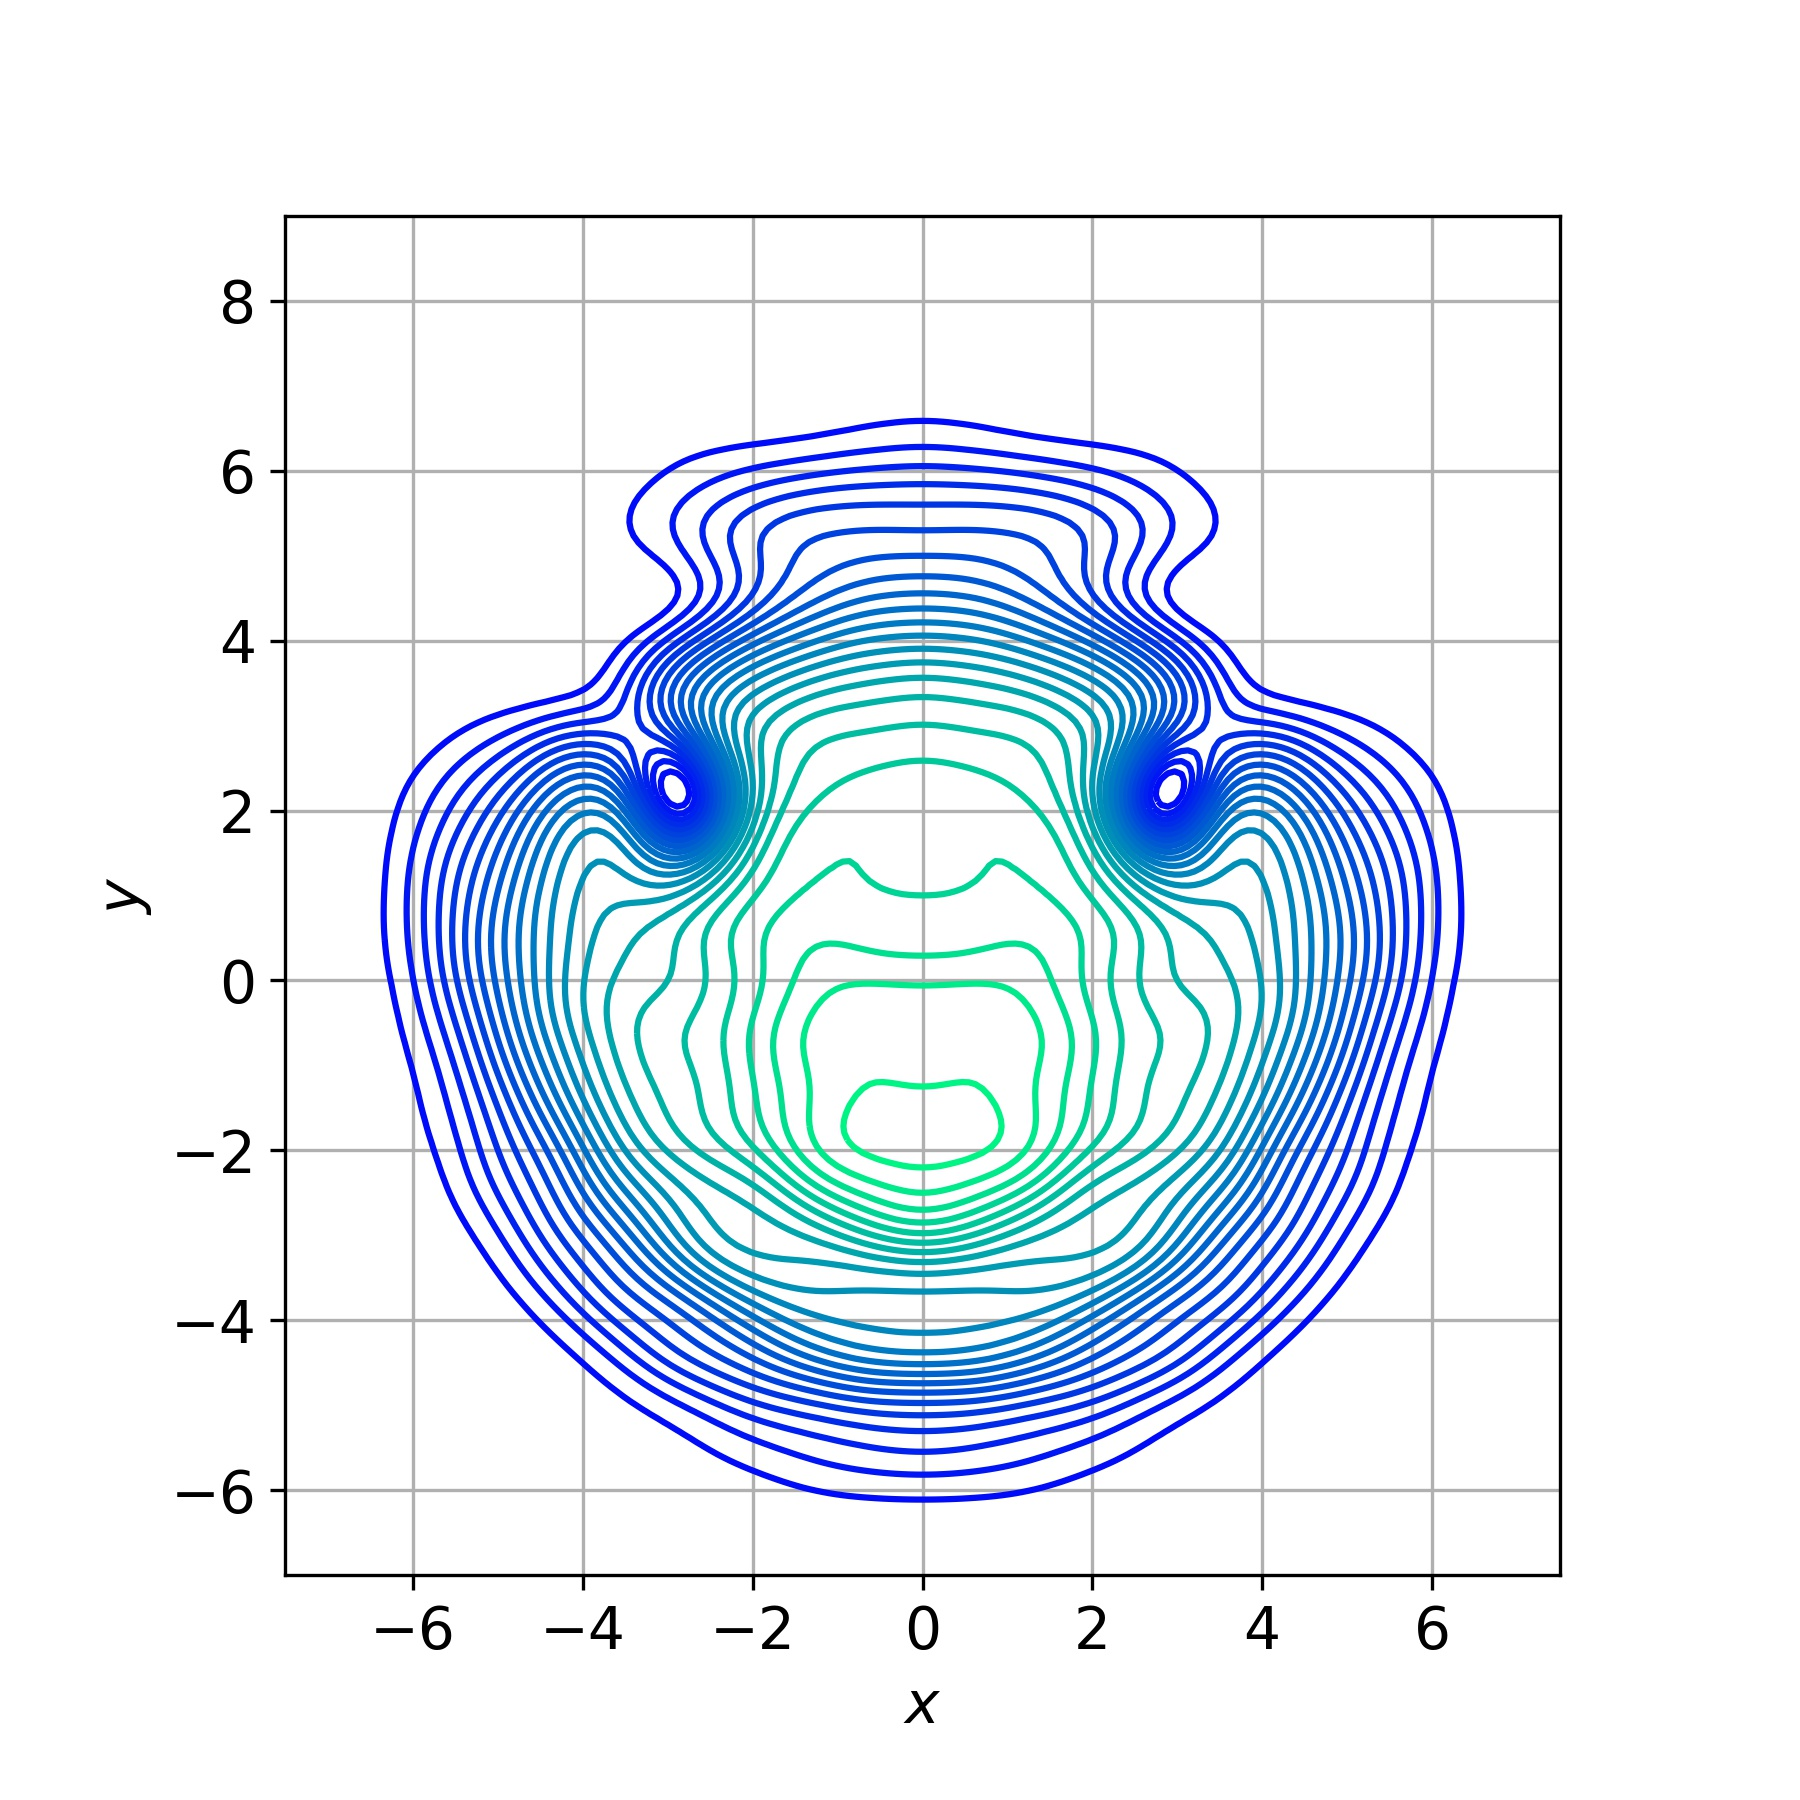
\includegraphics[width=\linewidth]{imgs/vortex_contour/contour_vortices_80.jpeg}
\caption{$t = 0.8$}\label{fig:gull}
\end{subfigure}
\begin{subfigure}[b]{.45\linewidth}
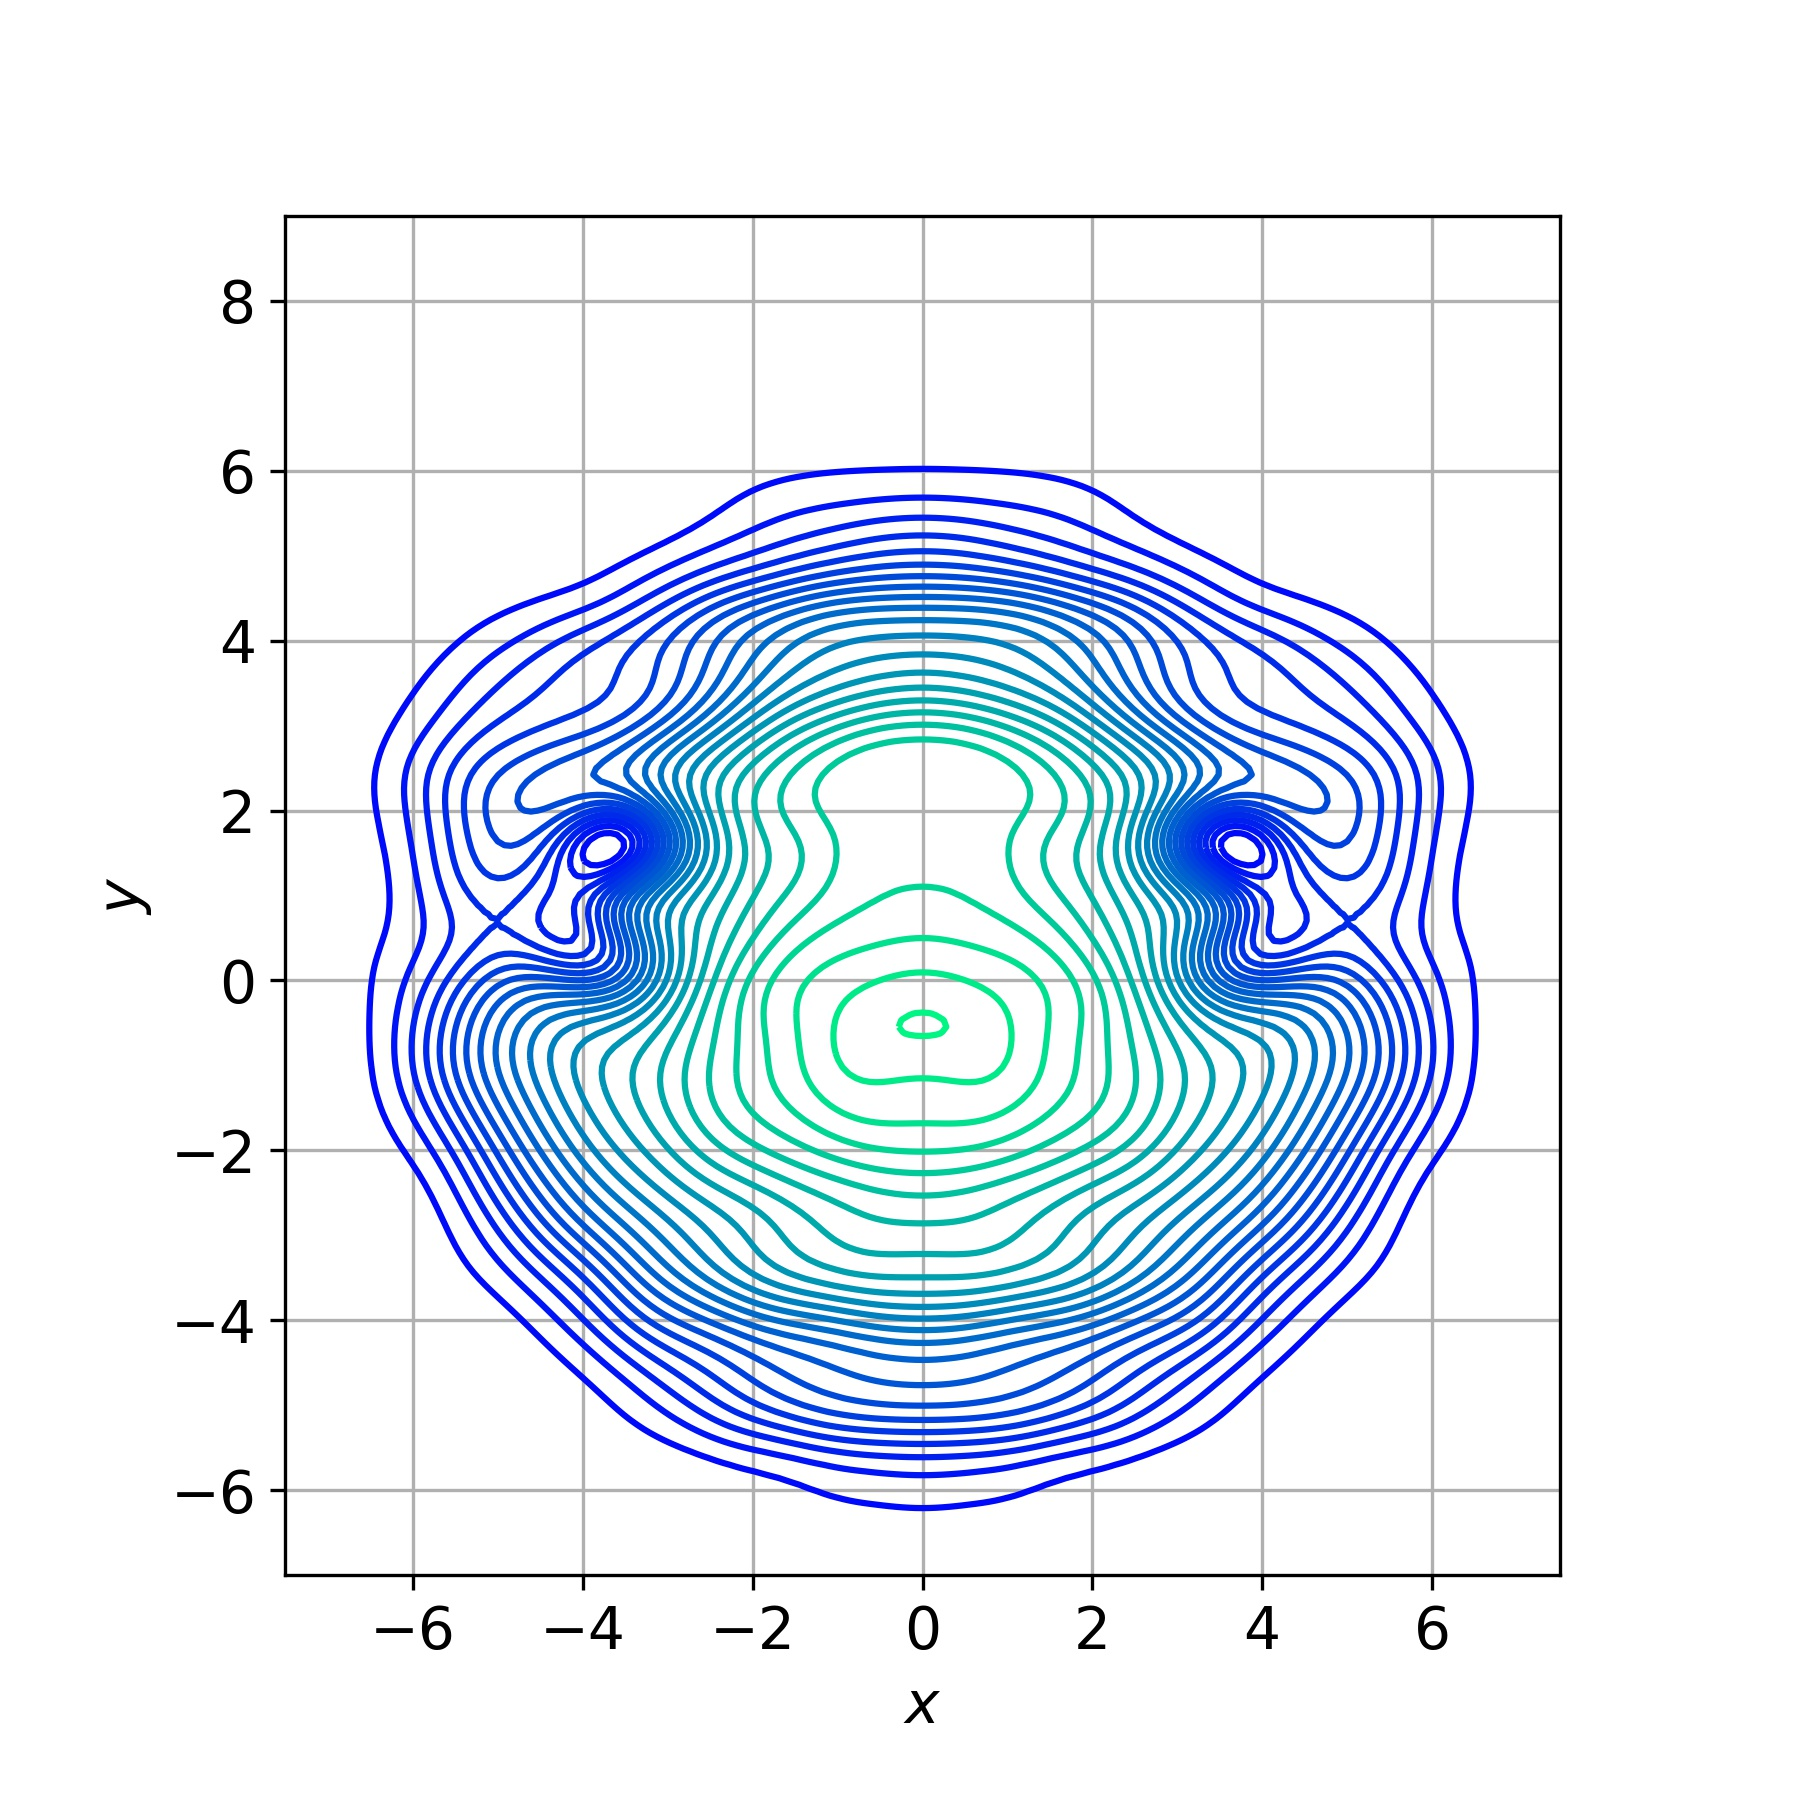
\includegraphics[width=\linewidth]{imgs/vortex_contour/contour_vortices_100.jpeg}
\caption{$t = 1.0$}\label{fig:tiger}
\end{subfigure}

\caption{Evolution of the ground state of the condensate for the passage of a laser beam. }
\label{fig:ground-state-laser}
\end{figure}

The first important result that we can see from the plots is that the simulation is capable of making appear a topological defect for the wave function in a time varying potential. Some frames of the evolution of the wave function can be found in Figure \ref{fig:ground-state-laser}. The program has been run with $\kappa = 500$, $w_0 = 30$ and $\delta = 3$, as thee example shown in \cite{Adams} which has the same shape.



\section{Conclusion}\label{sec:Conc}




\newpage
\section*{Appendix}\label{sec:Appendix}
\addcontentsline{toc}{section}{Appendix}

\subsection*{Derivation of the Gross-Pitaevskii Equation}
\addcontentsline{toc}{subsection}{Derivation of the Gross-Pitaevskii Equation}

\subsubsection*{Time-independent GPE}
We follow the derivation presented in \cite{Pethick}. Adopting a mean field approach we can assume a symmetrized product of single particle wave functions as the wave function of the many body system. Thus, in the fully condensate state, when all bosons are in the same single particle state $\psi(\mathbf{r})$ the $N$-particles wave function is:
\begin{equation} \label{basic}
 \Psi(\mathbf{r}_1,\mathbf{r}_2,...,\mathbf{r}_N)=\prod_{i=1}^{N}\psi(\mathbf{r}_i)
\end{equation}
where, as usual the single particle state is normalized. We additionally consider a localized system, so that the boundary in the computed integrals terms can be eliminated.\par
In \cite{Pethick}, it is shown that, in a gas with scattering length $a$, the effective interaction between two particles at low energies is a constant in the momentum representation, given by :
$$
 U_0=\frac{4 \pi \hbar^2a}{m}
$$
When translated into the coordinate space it represents a contact interaction:
$$
 U(\mathbf{r},\mathbf{r}')=U_0 \delta(\mathbf{r}-\mathbf{r}')
$$
where $\mathbf{r}$ and $\mathbf{r}'$ represent the position of the two particles. To take into account the effects of the interaction between two atoms when they are close to each other we should include this term in our Hamiltonian:
$$
 \hat{H}=\sum_{i=1}^N \left(\frac{\hat{p}_i^2}{2m}+V(\mathbf{r}_i)\right)+U_0\sum_{i<j}\delta(\mathbf{r}_i-\mathbf{r}_j)
$$
where $V(\mathbf{r})$ is the external potential.\par
Let us now consider the energy of the state \eqref{basic}:
\begin{equation}\label{En_Statev}
 E=\langle\Psi|\hat{H}|\Psi\rangle=\int d\mathbf{r}_1 d\mathbf{r}_2 ... d\mathbf{r}_N \Psi^{*}\hat{H}\Psi
\end{equation}
Let us compute it step by step. The interaction term is:
$$
\int  d\mathbf{r}_1 d\mathbf{r}_2 ... d\mathbf{r}_N \left( U_0\sum_{i<j}\delta(\mathbf{r}_i-\mathbf{r}_j)\prod_{k}\psi(\mathbf{r}_k)^{*}\psi(\mathbf{r}_k)\right)
$$
Clearly, the integral of each term of the sum is $\int d\mathbf{r}_i |\psi(\mathbf{r}_i)|^4$, due to normalization and to the integration properties of the $\delta$ function. The number of terms is $N(N-1)/2$, the number of pairs of two elements. So, the previous integral reduces to:
$$
 \frac{N(N-1)}{2}U_0\int d\mathbf{r}_i |\psi(\mathbf{r}_i)|^4
$$
The potential term would be:
$$
 \int d\mathbf{r}_i d\mathbf{r}_2 ... d\mathbf{r}_N\left(\sum_{i=1}^{N}V(\mathbf{r}_i)\prod_{j=1}^{N}\psi(\mathbf{r}_j)^{*}\psi(\mathbf{r}_j)\right)=N\int d\mathbf{r} V(\mathbf{r})|\psi(\mathbf{r})|^2
$$
Finally the momentum term is:
$$
 \int d\mathbf{r}_i d\mathbf{r}_2 ... d\mathbf{r}_N \left(\sum_{i=1}^{N}\left(-\frac{\hbar^2}{2m}\nabla^2\psi(\mathbf{r}_i)\psi(\mathbf{r}_i)^{*}\prod_{j\neq i}\psi(\mathbf{r}_j)^{*}\psi(\mathbf{r}_j)\right)\right)=N\int d\mathbf{r} \left(-\frac{\hbar^2}{2m}\nabla^2\psi(\mathbf{r})\psi(\mathbf{r})^{*}\right)
$$
Integrating by parts we get:
$$
 N\int d\mathbf{r} \left(\frac{\hbar^2}{2m}|\nabla\psi(\mathbf{r})|^2\right)
$$
Now, substituting the three terms into \eqref{En_Statev}, we get:
\begin{equation}\label{Energy_int}
 E=N\int d\mathbf{r}\left(\frac{\hbar^2}{2m}|\nabla\psi(\mathbf{r})|^2+V(\mathbf{r})|\psi(\mathbf{r})|^2+\frac{(N-1)}{2}U_0|\psi(\mathbf{r})|^4\right)
\end{equation}

In what follows, it is convenient to introduce the wave function of the condensate, given by 
$$
 \phi(\mathbf{r})=N^{1/2}\psi(\mathbf{r})
$$
so that the density of particles is given by:
$$
 n(\mathbf{r})=|\phi(\mathbf{r})|^2
$$
The equation \eqref{Energy_int} takes the form:
\begin{equation}\label{Energy_cond_wave_f}
 E=\int d\mathbf{r}\left(\frac{\hbar^2}{2m}|\nabla\phi(\mathbf{r})|^2+V(\mathbf{r})|\phi(\mathbf{r})|^2+\frac{1}{2}U_0|\phi(\mathbf{r})|^4\right)
\end{equation}
As we are looking for the zero temperature state, we have to minimize the energy with respect to $\phi(\mathbf{r})$ and $\phi^{*}(\mathbf{r})$ independently, under the constraint that the total number of particles remain constant: 
$$
 N=\int d\mathbf{r}|\phi(\mathbf{r})|^2
$$
So, we have to determine the condition which ensures:
$$
 \delta E- \mu \delta N=0
$$
where $\mu$ is just a Lagrange multiplier that in fact matches the chemical potential of a particle in the condensate. The previous equation results into an expression with two terms, one for the variation of $\phi$ and one for the variation of $\phi^*$. But in fact, once you consider one of them, the other provides no new information as it is its complex conjugate. So considering only the variation with respect to $\phi^*$:
$$
 \delta E-\mu \delta N \propto \int d\mathbf{r} \left(\frac{\hbar^2}{2m}\nabla( \delta \phi^*)\nabla \phi +V(\mathbf{r})\delta \phi^* \phi +U_0 |\phi(\mathbf{r})|^2 \phi(\mathbf{r})-\mu \phi(\mathbf{r}) \delta \phi^*\right)=0
$$
Integrating by parts the first term we get:
$$
 \delta E-\mu \delta N \propto \int d\mathbf{r}\delta \phi^* \left(\frac{-\hbar^2}{2m}\nabla^2 \phi(\mathbf{r}) +V(\mathbf{r}) \phi +U_0 |\phi(\mathbf{r})|^2 \phi(\mathbf{r})-\mu \phi(\mathbf{r})\right)=0
$$
This being true for arbitrary $\delta \phi^*$, we obtain the condition:
\begin{equation}\label{GP_Eq1}
 \left(\frac{-\hbar^2}{2m}\nabla^2 +V(\mathbf{r}) +U_0 |\phi(\mathbf{r})|^2 \right)\phi(\mathbf{r})=\mu \phi(\mathbf{r})
\end{equation}

This last equation is the time-independent GPE. It clearly has the form of a Schrödinger equation in the presence of a potential with a non-linear term $U_0|\phi(\mathbf{r})|^2$ which represents the mean field effect of the whole condensate over each individual member of the system of bosons. On the right hand side the eigenvalue of the equation is the chemical potential. In the case of non-interacting particles all in the ground state, it also represents the energy per particle.

\subsubsection*{Time-dependent GPE}
The time-dependent Gross-Pitaevskii Equation, describes the dynamics of the condensate in a first approximation. It is natural to generalize the previously obtained ``stationary Schrödinger equation'' and directly define the time-dependent GPE as a Schrödinger equation with the non-linear ``potential'': 
\begin{equation}\label{eq:almostGPE}
  i\hbar \frac{\partial \phi(\mathbf{r},t)}{\partial t}=\left(\frac{-\hbar^2}{2m}\nabla^2 +V(\mathbf{r},t) +U_0 |\phi(\mathbf{r},t)|^2 \right)\phi(\mathbf{r},t)  
\end{equation}
But just as the time-independent one, the latter can be derived from variational principles considering:
$$
 \delta \int_{t_1}^{t2}Ldt=0
$$
where $L$, is given by:
$$
  L=\int d\mathbf{r}\frac{i\hbar}{2}\left(\phi^*\frac{\partial \phi}{\partial t}-\phi \frac{\partial \phi^*}{\partial t}\right)-E =\int d\mathbf{r}\frac{i\hbar}{2}\left(\phi^*\frac{\partial \phi}{\partial t}-\phi \frac{\partial \phi^*}{\partial t}-\xi\right)
$$
where $\xi=\frac{\hbar^2}{2m}|\nabla\phi|^2+V(\mathbf{r})|\phi|^2+\frac{1}{2}U_0|\phi|^4$.

\bigskip \noindent
Substituting $\phi(\mathbf{r})=N^{1/2}\psi(\mathbf{r})$ in \eqref{eq:almostGPE}, we finally obtain our equation \eqref{eqGP}:
$$
i\hbar \pdv{\psi}{t} = -\frac{\hbar^2}{2m} \laplacian \psi + V \psi + U_0 N \abs{\psi}^2 \psi
$$

\newpage

\subsection*{Justification of the Strang Split for non-linear operators}
\addcontentsline{toc}{subsection}{Justification of the Strang split for non-linear operators}

This is almost a complete formal proof. It neglects however technical issues relating to uniformity in $\mathbf{x}$ of the error. Uniformity is indeed of practical value because this is what ensures that, for a small enough time-step, we can have the \textit{same} chosen precision on \textit{all} the points of our grid. The proof should also be completed by checking that the operators of the GPE satisfy the smoothness conditions.

\bigskip
Let $\mathcal{H}$ be a normed sub-vector space $\mathcal{F}(\mathbb{R}^n,\mathbb{C})$, $A$ and $B$ operators $\mathcal{H} \longmapsto \mathcal{H}$ (further smoothness hypotheses on $A$ and $B$ are given below), and $f:t\in \mathbb{R} \longmapsto f(t)\in \mathcal{H}$, such that (writing $f$ also for the function $(t,\mathbf{x}) \longmapsto f(t)(\mathbf{x})$):
\begin{equation}\label{initialEq}
    \partial_t f(t) = A(f(t)) + B(f(t))
\end{equation}
We want to prove that $f(t+\epsilon)=\varphi^{A+B}_{\epsilon}(f(t))=\varphi^A_{\epsilon/2}\circ\varphi^B_{\epsilon}\circ\varphi^A_{\epsilon/2}(f(t))+\mathcal{O}(\epsilon^3)$. The problem can be formulated this way. Let $f^{(1)},f^{(2)},f^{(3)}\in \mathcal{H}$ such that:
\begin{equation}\label{TSM}
\begin{split}
    \partial_t f^{(1)} &= A(f^{(1)})~~~~,~~~~ f^{(1)}(0)=f(t)\\
    \partial_t f^{(2)} &= B(f^{(2)})~~~~,~~~~ f^{(2)}(0)=f^{(1)}(\frac{\epsilon}{2})\\
    \partial_t f^{(3)} &= A(f^{(3)})~~~~,~~~~ f^{(3)}(0)=f^{(2)}(\epsilon)
    \end{split}
\end{equation}
We want to show that:
\begin{equation}\label{Theo}
    f(t+\epsilon)-f^{(3)}(\frac{\epsilon}{2}) ~=~ \mathcal{O}(\epsilon^3)
\end{equation}

For $\mathbf{x}\in \mathbb{R}^n$, we define the functionals $A_\mathbf{x} : g \longmapsto A(g)(\mathbf{x})\in \mathbb{C}$ and $B_\mathbf{x} : g \longmapsto B(g)(\mathbf{x})\in \mathbb{C}$. We will assume that for all $\mathbf{x}$, $A_\mathbf{x}$ and $B_\mathbf{x}$ are smooth enough so that their functional derivatives exist and they can be Taylor-expanded to the 2\textsuperscript{nd} order:
\begin{equation}\label{Taylor}
    F(g+\epsilon h)=F(g)+\epsilon\int d\mathbf{x}\fder{F}{g}(\mathbf{x}) h(\mathbf{x})+\frac{\epsilon^2}{2}\int d\mathbf{x}_1d\mathbf{x}_2 \fdder{F}{g}(\mathbf{x}_1,\mathbf{x}_2)h(\mathbf{x}_1)h(\mathbf{x}_2)+\mathcal{O}(\epsilon^3)
\end{equation}
for $F=A_\mathbf{x},B_\mathbf{x}$. It also follows that:
\begin{equation}\label{totalder}
    \frac{d}{dt}F(g(t))=\int d\mathbf{x}\fder{F}{g(t)}(\mathbf{x})~\partial_t g(t,\mathbf{x})
\end{equation}

\bigskip\noindent
\textit{Proof of} \eqref{Theo}

\bigskip
Let $\mathbf{x}_0\in\mathbb{R}^n$. We have:
$$f(t+\epsilon,\mathbf{x}_0)=f(t,\mathbf{x}_0)+\epsilon\partial_t f(t,\mathbf{x}_0)+\frac{\epsilon^2}{2}\partial_t^2 f(t,\mathbf{x}_0)+\mathcal{O}(\epsilon^3)$$
From \eqref{initialEq} and using \eqref{totalder} we get:
\begin{equation}\label{Eqf}
    \begin{split}
    f(t+\epsilon,\mathbf{x}_0)=&f(t,\mathbf{x}_0)~+~\epsilon (A_{\mathbf{x}_0}+B_{\mathbf{x}_0})(f(t))\\
    &+\frac{\epsilon^2}{2}\int d\mathbf{x}\left[ \fder{A_{\mathbf{x}_0}}{f(t)}(\mathbf{x})+\fder{B_{\mathbf{x}_0}}{f(t)}(\mathbf{x}) \right]~ (A_{\mathbf{x}_0}+B_{\mathbf{x}_0})(f(t))(\mathbf{x}) ~+~\mathcal{O}(\epsilon^3)
    \end{split}
\end{equation}
In the following we will drop the $\mathbf{x}_0$, keeping in mind that the equations have in fact the form of \eqref{Eqf}.\par
\noindent
Let us now compute $f^{(3)}(\frac{\epsilon}{2})$. We will use \eqref{TSM}, \eqref{Taylor} and \eqref{totalder} and keep only 2\textsuperscript{nd} order terms in $\epsilon$ at most.
\small
\begin{align*}
        f^{(3)}(\frac{\epsilon}{2})&=f^{(3)}(0)+\epsilon\partial_t f^{(3)}(0)+\frac{\epsilon^2}{8}\partial_t^2f^{(3)}(0)+\mathcal{O}(\epsilon^3)\\
        &= f^{(3)}(0) + \frac{\epsilon}{2}A(f^{(3)}(0)) + \frac{\epsilon^2}{8}\int \fder{A}{f^{(3)}(0)}A(f^{(3)}(0))~+~\mathcal{O}(\epsilon^3)
\end{align*}
\normalsize
We have {\scriptsize $f^{(3)}(0)=f^{(2)}(\epsilon)=f^{(2)}(0)+\epsilon\partial_t f^{(2)}(0)+\frac{\epsilon^2}{2}\partial_t^2f^{(2)}(0)+\mathcal{O}(\epsilon^3)$}. So, Taylor-expanding:
\small
\begin{align*}
        f^{(3)}(\frac{\epsilon}{2})&= f^{(2)}(0)+\epsilon\partial_t f^{(2)}(0)+\frac{\epsilon^2}{2}\partial_t^2f^{(2)}(0) + \frac{\epsilon}{2}\left(A(f^{(2)}(0)+\int \fder{A}{f^{(2)}(0)}\epsilon\partial_t f^{(2)}(0)\right)\\
        &\qquad \qquad \qquad+ \frac{\epsilon^2}{8}\int \fder{A}{f^{(2)}(0)}A(f^{(2)}(0)) ~+~\mathcal{O}(\epsilon^3)\\
        &=f^{(2)}(0)+\epsilon\left[B(f^{(2)}(0)+\frac{1}{2}A(f^{(2)}(0)\right]\\
        &\qquad +\frac{\epsilon^2}{2}\left[\fint{B}{f^{(2)}(0)}{B}+\fint{A}{f^{(2)}(0)}{B}+\frac{1}{4}\fint{A}{f^{(2)}(0)}{A}\right]~+~\mathcal{O}(\epsilon^3)
\end{align*}
\normalsize
Again we have {\scriptsize $f^{(2)}(0)=f^{(1)}(\frac{\epsilon}{2})=f^{(1)}(0)+\frac{\epsilon}{2}\partial_t f^{(1)}(0)+\frac{\epsilon^2}{8}\partial_t^2f^{(1)}(0)+\mathcal{O}(\epsilon^3)$}, so:
\small
\begin{align*}
        f^{(3)}(\frac{\epsilon}{2})&= f^{(1)}(0)+\frac{\epsilon}{2}\partial_t f^{(1)}(0)+\frac{\epsilon^2}{8}\partial_t^2f^{(1)}(0)\\&\qquad+ \epsilon\left(B(f^{(1)}(0))+\int \fder{B}{f^{(1)}(0)}\frac{\epsilon}{2}\partial_t f^{(1)}(0)+\frac{1}{2}A(f^{(1)}(0))+\frac{1}{2}\int \fder{A}{f^{(1)}(0)}\frac{\epsilon}{2}\partial_t f^{(1)}(0)\right)\\
        &\qquad \qquad + \frac{\epsilon^2}{2}\left(\fint{B}{f^{(1)}(0)}{B}+\fint{A}{f^{(1)}(0)}{B}+\frac{1}{4}\fint{A}{f^{(1)}(0)}{A}\right) ~+~\mathcal{O}(\epsilon^3)
\end{align*}
\normalsize
Gathering terms, we get:
\begin{equation}\label{Eqf3}
    \begin{split}
    f^{(3)}(\frac{\epsilon}{2})=& f^{(1)}(0)~+~\epsilon (A+B)(f^{(1)}(0))\\
    &+\frac{\epsilon^2}{2}\int \left[ \fder{A}{f^{(1)}(0)}+\fder{B}{f^{(1)}(0)} \right]~ (A+B)(f^{(1)}(0)) ~+~\mathcal{O}(\epsilon^3)
    \end{split}
\end{equation}
Since $f^{(1)}(0)=f(t)$, we see that the expression is the same as \eqref{Eqf}. Hence we proved \eqref{Theo}.

\bigskip
A similar computation shows that the simpler approximation $\varphi^A_\epsilon\circ\varphi^B_\epsilon(f(t))$ has en error of order $\epsilon^2$.


\newpage

\normalem
\bibliographystyle{acm}
\bibliography{ref}


\end{document}
